% !TEX TS-program = xelatex
% !BIB program = biber
% !TEX encoding = UTF-8 Unicode

% 使用手冊請見 TW_Thesis_Template wiki:
% https://github.com/sppmg/TW_Thesis_Template/wiki

% User guide in wiki of TW_Thesis_Template :
% https://github.com/sppmg/TW_Thesis_Template/wiki

\documentclass[oneside]{NCU_thesis} % \documentclass[option1, option2, ...]
% Helpful options: 
% draft = Don't load figure ,reduce compile time.
% showframe = show document margins.
% colorgrid = show colored coordinate. (by eso-pic pkg.)
\usepackage[subpreambles]{standalone} % standalone class setting in config.tex
% Option ``subpreambles'' enable sub-tex's preambles when compile main tex. (pkg default disable)
% sppmg think it's still some problem (e.g. \addbibresource will faild ), recommend move all subpreambles to ``macros_preamble.tex``

\begin{document}
    \frontmatter
        \documentclass[class=NCU_thesis, crop=false, float=true]{standalone}
\begin{document}
% I use LaTeX3 to automatically generate name table. 
% Below \ExplSyntaxOn to \ExplSyntaxOff perpare prof. table contents,
% it will save contents to `\profsTableContent''. 
% You can ignore this block even you want make table by yourself.
\ExplSyntaxOn
% Copy prof. list from config.tex
\clist_gclear_new:N \g_sppmg_profs_cl
\clist_gset:NV \g_sppmg_profs_cl \profs

% get total number of prof. . Omitted language will not display.
\int_gzero_new:N \g_sppmg_profTotal_int 
\int_gset:Nn \g_sppmg_profTotal_int {\clist_count:N \g_sppmg_profs_cl} 

% NOTE: ``tabularx'' will  processes its contents more than once
% for calculate width, so ``gpop'' can't put in tabularx env.
\tl_gclear_new:N \g_sppmg_tableContent_tl

% Use a inline function for pop list , and save table content 
% Input(#1) switch 3 case, 1 = Advisor, 2 = committee member , 3+ is more.
% Use ``for'' loop to get all prof.
\int_step_inline:nnnn {1}{1}{\g_sppmg_profTotal_int}{
    \clist_gpop:NNTF \g_sppmg_profs_cl \l_tmpa_tl {}{ \tl_clear:N \l_tmpa_tl}
    \tl_gput_right:Nx \g_sppmg_tableContent_tl {
        \int_case:nnTF {#1}{
            {1} {指導教授: & \l_tmpa_tl & 博士 \exp_not:n {\\} }
            {2} {共同指導: & \l_tmpa_tl & 博士 \exp_not:n {\\} }
        }{}{
             & \l_tmpa_tl & 博士 \exp_not:n {\\} 
        }
    }
}

% Copy contents to LaTeX2e macro.
\cs_set_eq:NN \profsTableContent \g_sppmg_tableContent_tl

\ExplSyntaxOff


\def\fsUniversity{\fontsize{26}{31}\selectfont }
\def\fsTitle{\fontsize{22}{26.4}\selectfont }
\def\fsNames{\fs{16}[1.5] }
% --------define title page layout for thesis
\titlepageFontFamily % set in config.tex
\newgeometry{top=2.5cm, bottom=2.5cm, inner=2cm, outer=2cm} % only for titlepage
\begin{spacing}{1.0}
\begin{titlepage}
    \null\vfill
    \begin{center}
        {\fsUniversity\textbf{國\quad 立\quad 中\quad 央\quad 大\quad 學}\par}
        \vspace*{20mm}
        
        {\fsTitle {\dept} \par}
        \vspace*{1ex}
        
        {\fsTitle {\degree}論文\par}
        \vspace*{20mm}
        
        {\fsTitle {\title} \par}
        \vspace*{5mm}
        
        {\fsTitle {\subtitle} \par}
        \vspace*{10mm}
        
        {\ifx \logo\empty\vspace*{40mm}
        \else \includegraphics[height=30mm]{\logo}\vspace*{10mm} \par
        \fi}
        \vfill
        
        {\fsNames \renewcommand{\arraystretch}{1}
            % If you want make table by yourself, replace ``\profsTableContent''
            \begin{tabular}{l@{\hspace*{0.4em}}l@{\quad}r}
                % 0.4em for ``:'' right side space
                研\enspace 究\enspace 生: & \author  &     \\
                
                \profsTableContent
                
            \end{tabular}
            \par
        }
        \vspace*{5ex}
        
        {\fsTitle {\degreedate} \par}
        \vspace*{2ex}
        
        \ifthenelse{\boolean{printcopyright}}
        {{{版權所有\copyright\ \author\ \copyyear} \par}}
    \end{center}
    \null\vfill
\end{titlepage}
\end{spacing}
\restoregeometry
\normalfont % use main font
%--------end of title page for thesis
\cleardoublepage
\end{document}
        % 封面/書名頁
        \listoftodos   % todo list, hide when set \textbackslash{}setboolean\{publish\}\{\textbf{true}\} in config.tex. It will not add to TOC , you can add \todototoc before \listoftodos to do that.
            % \todo[inline]{``Todo List'' will hide when set \textbackslash{}setboolean\{publish\}\{\emph{true}\} in config.tex.}

        %%%%%%%%%%%% letters %%%%%%%%%%%%
        % Set file name in config.tex
        % 碩博士論文電子檔授權書 Authorization Letter/Power of Attorney
        \IfFileExists{\letterAuthEl}{
            \cleardoublepage        % 由下個右頁開始
            \includepdf{\letterAuthEl}}{}
        % 碩博士紙本論文延後公開/下架申請書。(如需延後公開者,才需要裝訂於論文內頁)
        % \IfFileExists{\letterPubReq}{
        %     \cleardoublepage
        %     \includepdf{\letterPubReq}}{}
        % 指導教授推薦書
        \IfFileExists{\letterRecom}{
           \cleardoublepage
           \includepdf{\letterRecom}}{}
        % 口試委員審定書
        \IfFileExists{\letterVerif}{
            \cleardoublepage
            \includepdf{\letterVerif}}{}
        \cleardoublepage
        
        %%%%%%%%%%%% Other frontmatter, eg,abstract %%%%%%%%%%%%
        % 中英文論文摘要:內容應說明研究目的,資料來源,研究方法及研究結果等
        \documentclass[class=NCU_thesis, crop=false]{standalone}
\begin{document}

\chapter{摘要}
嬰兒照護者在照顧嬰兒時,
可能發生無法隨時關注嬰兒狀態的情形,
使得嬰兒因溢奶、翻身、趴睡等情形,
致使呼吸不順而發生憾事。
又因現有產品多用感測器偵測嬰兒狀態,
功能單一且多有使用限制,
便利性不佳。

因此,
本論文提出基於深度學習技術,
專注於嬰兒影像畫面之危險監測系統:
首先,
使用SSD演算法及RetinaFace演算法偵測嬰兒臉部;
接著,
利用ResNet50訓練模型,
用以辨識嬰兒臉部是否遭非奶嘴之異物遮蔽,
以及辨識四種基礎姿勢:正躺、趴躺、坐姿及站立。
故當系統輸入嬰兒影片時,
可透過模型辨識嬰兒的姿勢可能處於危險狀態或臉部遭異物遮擋,
則可即時警示照護者。

本文中,
利用SSD演算法偵測之時間優勢,
偵測每張影像平均僅需0.04秒,
且準確度達99\%;
使用RetinaFace演算法偵測嬰兒臉部雖需較長時間,
但其正確率、準確度及召回率皆達99\%;
而危險偵測之臉部遮擋辨識模型及姿勢辨識模型,
其準確度亦皆達99\%。

另外,
由於目前未有公開之嬰兒資料集,
本文中所使用的嬰兒照片皆為網路真實嬰兒圖片及影片,
進行前處理收集而成。

\vspace{2em}
\noindent \textbf{關鍵字:} \keywordsZh{} % Set keywords in config.tex
\end{document} % zh 中文摘要
        \documentclass[class=NCU_thesis, crop=false]{standalone}
\begin{document}

\chapter{Abstract}
The babysitter may not focus on the status of the infant at any time.
When unpredictable things happen to the baby, such as spitting up, rolling over, or sleeping on his stomach, 
the babysitter won't notice immediately. 
Most of the existing products are sensor-based infant detection systems, 
which are single-function and may disturb the movement of the baby.
However, the existing vision-based infant detection studies only focus on breathing rate, facial features, and individual movements.

Therefore, this paper proposes a danger monitoring system based on deep learning technology.
The system focuses on baby images and includes two major functions:
(1) Facial Occlusion Recognition: Determine whether the infant's face is occluded by foreign objects, which may cause suffocation.
(2) Posture Recognition: The four basic postures of infants are analyzed: lying on the back, lying on the stomach, sitting and standing.
If the baby is lying on his stomach or standing, he may be at risk of breathing difficulties or falling off the bed.
In summary, while monitoring the baby's video, the system can alert the babysitter when the infant is in an alarm state.

In this study, infant face detection uses the faster execution time SSD algorithm and the higher performance RetinaFace algorithm.
With these algorithms, the system strikes a balance between execution speed and accuracy.
There is currently no open source infant dataset.
Therefore, this paper collects real baby images and videos from different perspectives from the Internet to create an infant face dataset with 3475 images and an infant posture dataset with 15416 images.
Then, two models of face occlusion recognition and posture recognition are trained using ResNet50, 
and the training and testing accuracy are 99\%.
This proves that this study has good utility and uniqueness for infant danger monitoring system.

\vspace{2em}
\noindent \textbf{Keywords:} \keywordsEn{} % Set keywords in config.tex
\end{document} % en 英文摘要
        \documentclass[class=NCU_thesis, crop=false]{standalone}
\begin{document}

\chapter{誌謝}

就讀碩士班期間,接受了很多人的幫助與鼓勵,
非常感謝這兩年的所有時光。

首先,感謝蘇木春老師的指導,
在研究上給予了我很多的方向與教學,
讓我能在碩士期間獲益良多;
也感謝蘇老師很信任學生,
讓我在這兩年得以很好的妥善規劃時間。

接著,感謝實驗室的每位成員,
讓我在CILAB擁有這麼珍貴的回憶。
感謝佳菁、小花、熙琪、小烏龜,
處理實驗室繁忙的事務,讓我們可以有這麼舒適的研究環境;
感謝威任學長、偉倫學長,
在研究中提供了很多想法,讓我在研究中能有更明確的方向;
感謝子謙學長、政育學長、映如學姊、書伃學姊,
在我有疑惑的時候,解答了許多的問題,帶領我們熟悉實驗室的生活;
感謝鈞翔、昌翰、逸星、奕蘋、詩勻,
交流彼此的意見與想法,讓我能激發出更多不同的思維;
感謝智穎、景豐、季劫、譽鈞、姿瑩,
一起參與了許多實驗室的事務,讓所有活動及計畫得以完成。

最後,也感謝我的家人、朋友、愛人以及我自己,
在不同的人生階段中一起度過,
給予我非常多的支持與幫助,
而得以逐漸成長為一位更成熟的個體。

\end{document}


 % 誌謝(可略)

        % 論文相似度比對報告電子回條
        %\IfFileExists{\letterThesisSim}{
        %    \cleardoublepage
        %    \includepdf{\letterThesisSim}}{}
        % 學術倫理修課證明
        %\IfFileExists{\letterCareCert}{
        %    \cleardoublepage
        %    \includepdf{\letterCareCert}}{}
        % 遠距口試申請
        %\IfFileExists{\letterRemoteExam}{
        %    \cleardoublepage
        %    \includepdf{\letterRemoteExam}}{}

        % 原始 book class 不將 TOC,LOF,LOT 加入目錄列表,須手動加
        % 此樣板可由 config.tex 切換是否自動加入目錄
        \tableofcontents        % 目錄
        \listoffigures          % 圖目錄
        \listoftables           % 表目錄
        %\documentclass[class=NCU_thesis, crop=false]{standalone}
\begin{document}

\chapter{使用符號與定義}
這裡示範用表格做符號與定義列表。你也可以利用套件``nomencl''(簡易)或``glossaries''(強大)完成,詳細說明見教學(v1.8+)。

\begin{table}[h]
    \normalsize % 使用與內文一樣大的字體,請自調
    \centering
    \begin{tabular}{c@{\quad:}l}
%         符號     & 說明 \\ 
        VIM     & 用vim的是神 \\ 
        Emacs   & 神在用的編輯器 \\ 
        CTAN    & Comprehensive TeX Archive Network, ctan.org \\
        
    \end{tabular} 
    \caption*{符號與定義} % 不想顯示請註解/刪除\caption行(\label自動失效)
    \label{table:symbol_def}
\end{table}

\end{document}
    % 符號說明
    \mainmatter
        \documentclass[class=NCU_thesis, crop=false]{standalone}
\begin{document}

\chapter{緒論}
\section{研究動機}
根據衛生福利部統計處所發布的嬰兒主要死因統計
~\cite{__2021}
中,
101年至105年間每年至少30位嬰兒死於嬰兒猝死症候群(Sudden infant death syndrome,簡稱SIDS),
106年至109年每年亦仍有超過20位嬰兒因此症狀逝世,
是為嬰兒十大死亡原因之一。

三軍總醫院對於嬰兒猝死症的說明為:
一個原本無異狀的嬰兒,突然且無法預期的死亡,
常發生在嬰兒睡眠時,並在事後的屍體解剖檢查中找不到其真正致死原因。
凡未滿一歲的嬰幼兒皆可能發生,其中二至四個月時期尤為常見,
亦可能發生在嬰兒出生一至兩周內。
醫界雖持續探討嬰兒猝死症的發生原因,
但目前對於真正的成因仍不清楚,
綜合醫界當前相關因素的研究中,
包含了嬰兒因溢奶或嘔吐產生呼吸道緊縮反射及憋氣,
或因翻身、趴睡致使呼吸困難,
而窒息死亡等原因。

當照護者在嬰兒照護時,
可能有許多不可避免的情形,
而難免發生視線離開嬰兒的情形,
如:泡奶、做飯、上廁所等,
進而無法百分之百關注嬰兒的各種行為。
而若此時嬰兒發生溢奶、物品遮蓋口鼻、自行翻身或站立等情形,
將造成嬰兒處於危險情境中,
而可能導致憾事發生。

國內外有許多為自動化監測嬰兒狀態之研究,
主要包含兩種偵測方式:
其一為使用感測器量測嬰兒之特定生理訊號,
如:心率、呼吸頻率、體溫、身體位置或方向及嬰兒周圍之氣體濃度等,
透過收集到的數值以判定所監測之嬰兒處於正常狀態與否;
然而,使用此種監測方式具功能單一性,
若欲偵測其他生理訊號,則需增設更多不同種類的感測器,
不僅可能影響嬰兒之活動,亦可能產生更多潛在的危險性,
如:裝置纏繞嬰兒、孩童誤食裝置等。
其二為透過電腦視覺偵測嬰兒影像,
判定嬰兒是否處於危險狀態,
而現有研究中多僅針對嬰兒之面部特徵或單一狀態進行偵測;
然而,我們認為一張嬰兒影像包含了許多資訊得以應用,
如:同時偵測嬰兒面部及姿勢等,
則可透過影像偵測更廣泛的監測嬰兒不同危險情境。

因此,本論文開發出一透過嬰兒影像辨識其基礎姿勢與面部狀態,
以監測嬰兒是否因姿勢不適當或面部遭異物遮擋,
處於危險情境中而需警示照護者。
此方法不僅擁有可監測多種不同危險情境之優點,
亦可減少感測器式偵測將干擾嬰兒之缺點,
且對於未來欲增加其他監測功能有良好的擴充性。

\section{研究目的}
本論文基於深度學習技術,
利用ResNet50網路進行嬰兒動作及臉部遮擋之模型訓練,
且以DeepFace演算法前處理影像擷取出嬰兒臉部畫面,
而得以對嬰兒進行危險監測。

本研究預計達成以下目標:
\begin{itemize}
    \item 針對嬰兒姿勢部分,辨識嬰兒之正躺、趴睡、坐姿及站立之四項基礎姿勢,進而判斷嬰兒是否做出具危險之動作。
    \item 針對嬰兒臉部部分,判斷嬰兒是否因嘔吐物、毛巾等非奶嘴之外物遮蓋其面部,而可能使嬰兒發生窒息危險。
\end{itemize}

綜上目標,本論文將建構出一可對嬰兒姿勢及臉部遮擋進行危險監測之系統。

\section{論文架構}
本論文分為五個章節,其架構如下:

第一章、緒論,敘述本論文之研究動機、研究目的及論文架構。

第二章、相關研究,
敘述嬰兒猝死症之定義,
並探討近年與嬰兒監測相關之研究以及深度學習模型架構與面部辨識網路。

第三章、研究方法,
說明本研究之詳細內容,如:資料集之分類定義及前處理、以及完整系統之流程說明。

第四章、實驗設計與結果,
說明各項實驗設計內容以及評估方法,並對於實驗結果進行探討。

第五章、結論與未來展望,
對於研究結果進行總結,並討論研究的未來展望。

\end{document}

    % 緒論
        \documentclass[class=NCU_thesis, crop=false]{standalone}
\begin{document}

\chapter{相關研究}

\section{嬰兒猝死症}
嬰兒猝死症(The Sudden Infant Death Syndrome, 簡稱SIDS)~\cite{kinney_sudden_2009}
其特徵為一位看似健康的嬰兒在睡眠期間突然死亡,
其真正致死之原因尚不明確且非單一。

目前醫界對嬰兒猝死症之直接致死原因尚未有統一的定義,
但可統整出多項促使此症發生之風險因素,
主要可分為兩類:
其一為外在因素,包含嬰兒因俯臥及側睡姿勢、蓋住臉部的床單、嬰兒睡在沙發或其他容易陷入的柔軟家具上等
~\cite{willinger_infant_1994, mitchell_reduction_1994, iyasu_risk_2002, kemp_unsafe_2000, ponsonby_factors_1993},
致使嬰兒呼吸困難而死亡;
其二則為內在因素,包含發展因素(如:早產~\cite{horne_effects_2006})、
遺傳因素(如:家族性之嬰兒猝死症~\cite{ce_sudden_2001, oyen_population-based_1996})、
性別(男性比例為女性的兩倍)或種族~\cite{hauck_sleep_2003}等。
除此之外,嬰兒也可能因其他外在環境條件,
如:產前或產後暴露於不良物質中(如:香菸煙霧、酒精或非法藥物等),
而弱化嬰兒之內在條件。

在嬰兒猝死症研究中,
有許多關於此症之死亡機制理論,
其中心肺控制假說主導了多數研究,
也造就了往後關於此症之探討多基於嬰兒呼吸或自主神經機制的缺陷。
此論點主要包含了五個步驟~\cite{kinney_sudden_2009}:
(1)發生危及生命的事件(如:面部朝下~\cite{kemp_sudden_1991}或面部遭遮蔽~\cite{skadberg_consequences_1997},造成反射性或阻塞性呼吸暫停),
而將導致嬰兒窒息或腦部灌注不足,亦可能兩者皆發生。
(2)嬰兒無法自行轉頭,以應對窒息的情境,而導致無法從呼吸暫停中恢復。
(3)持續性窒息導致嬰兒失去意識或反射,即低氧昏迷。
(4)發生心率過緩及缺氧喘氣,此現象在嬰兒因嬰兒猝死症逝世前將明顯發生。
(5)嬰兒的自主復甦能力受損,即因無效的喘氣而最終導致呼吸暫停及死亡。
因此,由嬰兒猝死症之紀錄中,
可看出此症並非一種突發疾病,
而是在嬰兒死亡前,
即會出現心率不正常或呼吸暫停之惡性循環現象。

另外,
亦有研究人員使用Triple-Risk Model來解釋嬰兒猝死症~\cite{noauthor_what_nodate},
即嬰兒死於此症需同時包含以下三個因素:
(1)有風險的嬰兒:嬰兒含有一個未知的問題,可能是基因突變或腦部缺陷等,這使其面臨了嬰兒猝死症的風險;
(2)嬰兒發育的重要時期:嬰兒出生後的前六個月,將經歷許多快速成長的階段,此階段會改變身體控制和調節自身的能力,且嬰兒的身體也會於此時學習如何對環境做出應變;
(3)環境中的壓力源~\cite{moon_sids_2011}:即前述中之外在因素,包含嬰兒睡姿及接觸香菸煙霧等。
若僅發生其中一項因素,
將不足以導致嬰兒猝死症引發死亡。

因此,
若能消除環境中的壓力源,
將有利於嬰兒的生存。
同時醫界亦發現俯臥睡姿勢將使嬰兒猝死症風險增加三倍以上~\cite{willinger_infant_1994},
故在1990年代初期國際間即提倡嬰兒仰臥睡姿,
此症之發病率也因此降低了50\% 以上,
但仍為嬰兒主要死亡原因之一。

\section{嬰兒監測系統}
在照護嬰兒的過程中,
由於嬰兒尚未發展出語言能力表達自己的不適,
或尚無能力將自己避免於危險之外。
因此,為了協助照顧者關注嬰兒狀態,
現有許多為自動化監測嬰兒之研究,
主要分為以感測器偵測生理訊號及以影像式偵測兩種方式。
% 兩種方式的優缺點比較

\subsection{感測器偵測}
此種方式利用多種不同感測器進行生理訊號之偵測,
包含利用呼吸感測器、濕度感測器、溫度感測器、非接觸式紅外溫度感測器、三軸加速度計、慣性感測器、一氧化碳感測器、二氧化碳感測器等,
分別量測嬰兒之呼吸頻率、出汗狀況、體溫、心率、身體位置或方向、睡眠姿勢、嬰兒周圍的一氧化碳濃度、呼出的二氧化碳濃度的變化等,
且多會透過物聯網技術開發出可穿戴式裝置之系統~\cite{klingeberg_mobile_2012, zhou_low_2015, bouwstra_smart_2009, malhi_zigbee-based_2012}。

如:
Linti等人~\cite{linti_sensory_2006}
所開發的嬰兒感測背心(\cref{fig:fig-linti_sensory_2006-01}),
其將多個感官元件融入紡織品中以用來量測嬰兒之呼吸、心率、溫度及濕度;
\fig[0.8][fig:fig-linti_sensory_2006-01][!hbt]{fig-linti_sensory_2006-01.png}[嬰兒多感測器背心之穿脫示意圖~\cite{linti_sensory_2006}][嬰兒多感測器背心之穿脫示意圖]
Ferreira等人~\cite{ferreira_smart_2016}
開發了將心律感測器、3D加速度計~\cite{hung_estimation_2008, pitts_respiratory_2013, bates_respiratory_2010}、
熱電堆感測器裝設於胸帶中(\cref{fig:fig-ferreira_smart_2016-01}),
而得以量測嬰兒之體溫、心率、呼吸頻率及身體位置,
並透過ZigBee技術將收集到的數據傳送至伺服器,
用戶則可透過醫療網頁介面進行查看及收到緊急訊息;
\fig[0.8][fig:fig-ferreira_smart_2016-01][!hbt]{fig-ferreira_smart_2016-01.png}[嬰兒穿戴式感測器裝置圖~\cite{ferreira_smart_2016}][嬰兒穿戴式感測器裝置圖]
Ziganshin等人~\cite{ziganshin_uwb_2010}
基於超寬頻技術開發出可監測嬰兒呼吸及心率之系統,
其可檢測嬰兒之睡眠狀態(\cref{fig:fig-ziganshin_uwb_2010-01})、
清醒狀態及警示狀態(\cref{fig:fig-ziganshin_uwb_2010-02});
\fig[0.8][fig:fig-ziganshin_uwb_2010-01][!hbt]{fig-ziganshin_uwb_2010-01.png}[嬰兒正常狀態之呼吸及心跳圖~\cite{ziganshin_uwb_2010}][嬰兒正常狀態之呼吸及心跳圖]
\fig[0.8][fig:fig-ziganshin_uwb_2010-02][!hbt]{fig-ziganshin_uwb_2010-02.png}[嬰兒呼吸暫停狀態之呼吸及心跳圖~\cite{ziganshin_uwb_2010}][嬰兒呼吸暫停狀態之呼吸及心跳圖]
Lin等人~\cite{lin_wireless_2014}
開發出一套在嬰兒胸帶上嵌入了三種不同感測器的系統(\cref{fig:fig-lin_wireless_2014-01}),
透過三軸加速度計可確定嬰兒睡姿(面朝上、下、左或右)與計算z軸資訊得出呼吸頻率(\cref{fig:fig-lin_wireless_2014-02})、
利用溫度感測器量測體溫以及使用一氧化碳感測器偵測嬰兒周圍之一氧化碳濃度,
再藉由WiFi模組傳送收集之生理資料至伺服器,
而其驗證所計算之呼吸頻率準確率達100\%。
\fig[0.8][fig:fig-lin_wireless_2014-01][!hbt]{fig-lin_wireless_2014-01.png}[嬰兒監測系統架構圖~\cite{lin_wireless_2014}][嬰兒監測系統架構圖]
\fig[0.8][fig:fig-lin_wireless_2014-02][!hbt]{fig-lin_wireless_2014-02.png}[z軸顯示吸氣及呼氣脈衝~\cite{lin_wireless_2014}][z軸顯示吸氣及呼氣脈衝]

此種利用感測器監測嬰兒的方法,
雖然可直接量測嬰兒之生理訊號以判斷狀態正常與否,
但仍可能因硬體設備之缺陷無法準確量測,
進而有失判斷準確性,
亦或者因嬰兒需額外穿戴裝置而造成不適,
進而影響嬰兒活動或導致更多危險的發生。

\subsection{影像式偵測}
此種方式利用電腦視覺技術對於嬰兒影像畫面進行偵測,
現有研究中包含了計算嬰兒之呼吸頻率、關注於嬰兒之面部特徵及嬰兒趴睡姿勢偵測。

Fang等人~\cite{fang_vision-based_2015}
開發了一基於視覺之非接觸式呼吸頻率偵測系統,
其系統流程為(見\cref{fig:fig-fang_vision-based_2015-01}):
先判斷嬰兒是否正在運動(包含頭部、四肢及身體運動,但不包含因呼吸引起的輕微運動,其判斷流程圖見\cref{fig:fig-fang_vision-based_2015-02}),
若未偵測到嬰兒運動,
則系統開始進行呼吸頻率偵測:
首先,透過空間特徵擷取呼吸之候選點;
接著,利用模糊積分技術選擇呼吸點;
最終,得以計算嬰兒的呼吸頻率,進而可判斷嬰兒是否發生呼吸異常之情形。
\fig[0.8][fig:fig-fang_vision-based_2015-01][!hbt]{fig-fang_vision-based_2015-01.png}[嬰兒呼吸頻率偵測系統流程圖~\cite{fang_vision-based_2015}][嬰兒呼吸頻率偵測系統流程圖]
\fig[0.8][fig:fig-fang_vision-based_2015-02][!hbt]{fig-fang_vision-based_2015-02.png}[嬰兒運動偵測流程圖~\cite{fang_vision-based_2015}][嬰兒運動偵測流程圖]

Liu等人~\cite{liu_video-based_2017}
利用夜視攝影機拍攝在嬰兒床內的嬰兒,
並使用MIT所提出之Eulerian Magnification技術,
放大影片中的細微運動以監測拍攝對象之胸部運動,
若經正規化之像素差異值低於設定閥值,
則判斷其呼吸頻率異常,
進而透過手機裝置發出警報。
系統整體設計圖見\cref{fig:fig-liu_video-based_2017-01}。
\fig[0.8][fig:fig-liu_video-based_2017-01][!hbt]{fig-liu_video-based_2017-01.png}[系統設計圖~\cite{liu_video-based_2017}][系統設計圖]

Gallo等人~\cite{gallo_marrsids_2019}
提出一名為MARRSIDS的模型,
其利用OpenCV之Haar-Like Features偵測嬰兒之面部特徵。
系統透過嬰兒臉部辨識與否及睜眼狀態,
判斷其是否處於危險情境中,
而需發出聲音警示:
若臉部未被偵測,
則認為嬰兒可能位於不良姿勢需發出警示;
而若嬰兒為睜眼狀態,
則代表嬰兒處於清醒狀態,
並非處於風險中。
系統之硬體架構圖見\cref{fig:fig-gallo_marrsids_2019-01},
人工視覺模型架構見\cref{fig:fig-gallo_marrsids_2019-02}。
\fig[0.8][fig:fig-gallo_marrsids_2019-01][!hbt]{fig-gallo_marrsids_2019-01.png}[硬體架構圖~\cite{gallo_marrsids_2019}][硬體架構圖]
\fig[0.8][fig:fig-gallo_marrsids_2019-02][!hbt]{fig-gallo_marrsids_2019-02.png}[人工視覺模型架構圖~\cite{gallo_marrsids_2019}][人工視覺模型架構圖]

Wang等人~\cite{wang_multi-task_2019}
提出了一個多任務貝氏深度神經架構(\cref{fig:fig-wang_multi-task_2019-01}),
其使用MobileNetV2網路,
針對自行收集之YunInfants資料集進行嬰兒頭部影像分析,
包含了四項子任務以達成嬰兒面部遮擋之監測:
(1)眼睛、鼻子或嘴巴是否可見,
(2)不可見的原因是否為被外物(如:枕頭)遮擋,
(3)眼睛睜開與否,
及(4)五個臉部座標之位置。
\fig[0.8][fig:fig-wang_multi-task_2019-01][!hbt]{fig-wang_multi-task_2019-01.png}[網路架構~\cite{wang_multi-task_2019}][網路架構]

Bharati等人~\cite{bharati_efficient_2021}
提出一個基於卷積神經網絡的電腦視覺系統,
可用來評估嬰兒三種睡眠姿勢(\cref{fig:fig-bharati_efficient_2021-01}):
仰臥(正常狀態)、從仰臥轉換到趴臥(警示狀態)、趴臥(危險狀態),
並於嬰兒呈現趴臥姿勢時,
透過手機提醒照護人員。
而此系統亦提供了驗證反饋機制,
供照護人員對於系統警報是否誤報之回饋。
另外,由於目前未有公開之嬰兒姿勢資料集,
此文透過拍攝和真實嬰兒相同比例之娃娃進行資料收集。
此研究之CNN架構見\cref{fig:fig-bharati_efficient_2021-02},
而系統完整架構見\cref{fig:fig-bharati_efficient_2021-03}。
\fig[0.8][fig:fig-bharati_efficient_2021-01][!hbt]{fig-bharati_efficient_2021-01.png}[睡姿分類~\cite{bharati_efficient_2021}][睡姿分類]
\fig[0.8][fig:fig-bharati_efficient_2021-02][!hbt]{fig-bharati_efficient_2021-02.png}[CNN架構~\cite{bharati_efficient_2021}][CNN架構]
\fig[0.8][fig:fig-bharati_efficient_2021-03][!hbt]{fig-bharati_efficient_2021-03.png}[系統架構~\cite{bharati_efficient_2021}][系統架構]

現有研究中,
多關注於嬰兒呼吸運動、面部特徵或單一姿勢偵測,
而尚未有對於嬰兒常見動作之辨識模型,
故我們提出一可偵測嬰兒基礎姿勢及面部遮擋之危險監測系統。

\section{ResNet}
過往神經網路訓練中,
更深層的網路會有模型退化的問題,
亦即隨著網路深度的增加,準確率達飽和後,反而迅速下降,
而這樣的結果並非因過度擬合所致,
如\cref{fig:fig-training-error}可看到兩個不同層數的網路其訓練誤差值。
\fig[1][fig:fig-training-error][!hbt]{fig-plain-network.png}[網路深度與訓練誤差關係][網路深度與訓練誤差關係]

因此,He等人~\cite{he_deep_2016}
提出了一個深度殘差學習(\cref{fig:fig-residual-learning})的架構,
利用shortcut connection執行identity mapping,
如此並不需要增加額外的參數,
亦即不增加計算複雜度。最終,本研究以152層的殘差網路在ILSVRC 2015中獲得第一名,
此網路比VGG網路深八倍,
卻仍擁有較低的複雜度。
\fig[0.8][fig:fig-residual-learning][!hbt]{fig-residual-learning.png}[殘差學習~\cite{he_deep_2016}][殘差學習]

\section{人臉偵測演算法}
\subsection{MTCNN}
MTCNN~\cite{zhang_joint_2016}
是由Zhang等人於2016年提出的一種多任務級聯卷積神經網路,
可以同時處理人臉偵測及對齊任務;
並提出可提升效能的online hard sample mining策略,
其是否使用之效能差距如\cref{fig:fig-mtcnn-online-hard-sample-mining}。
\fig[0.8][fig:fig-mtcnn-online-hard-sample-mining][!hbt]{fig-mtcnn-online-hard-sample-mining.PNG}[使用online hard sample mining策略效能比較~\cite{zhang_joint_2016}][使用online hard sample mining策略效能比較]

此網路包含三階段級聯架構的深度卷積網路,
以粗到細的方式預測人臉及座標位置,
其方法流程見\cref{fig:fig-mtcnn-pipeline}:
\fig[0.8][fig:fig-mtcnn-pipeline][!hbt]{fig-mtcnn-pipeline.PNG}[MTCNN pipline~\cite{zhang_joint_2016}][MTCNN pipline]
第一階段,
由全卷積網路構成之proposal network(P-Net)獲得人臉區域的候選窗口及其邊界框回歸向量,
並根據此估計回歸向量校準候選者,
再以nonmaximum suppression(NMS)合併高度重疊的候選者;
第二階段,
所有候選者皆饋送至另一個稱為refine network(R-Net)的CNN,
其進一步拒絕大量錯誤候選者,
並使用邊界框回歸進行校準及NMS;
第三階段,
則利用output network(O-Net)輸出五個臉部的座標位置,
其類似於第二階段,
但不同處是為識別具有更多監督的人臉區域。
此三階段網路的架構見\cref{fig:fig-mtcnn-framework},
圖中"MP"為max pooling、"Conv"為convolution,
而pooling及convolution的步長分別為2及1。
\fig[1][fig:fig-mtcnn-framework][!hbt]{fig-mtcnn-framework.PNG}[MTCNN framework~\cite{zhang_joint_2016}][MTCNN pipline]

\subsection{RetinaFace}
RetinaFace~\cite{deng_retinaface_2020}
是由Deng等人於2020年提出的single-shot、multi-level人臉定位方法,
其基於影像平面之點回歸整合了人臉框預測、2D人臉標示定位及3D頂點回歸。

此模型架構(見\cref{fig:fig-retinaface-framework})中,主要由三個部分組成:
(1)feature pyramid network、(2)context head module及(3)cascade multi-task loss。
首先,feature pyramid network獲得輸入影像,並輸出五個不同比例的特徵圖;
接著,context head module獲得這些特徵圖以計算多任務的損失:
亦即第一個模組會從一般的anchor預測範圍框,
而後第二個模組利用第一個模組迴歸出的anchor以預測更精準的範圍框。
\fig[1][fig:fig-retinaface-framework][!hbt]{fig-retinaface-framework.PNG}[RetinaFace架構~\cite{deng_retinaface_2020}][RetinaFace架構]

本篇論文展示了RetinaFace和其他29種人臉偵測演算法之平均準確度(Average Precision)比較,
如\cref{fig:fig-retinaface-ap}所示,
此演算法擁有91.7\%的良好結果。
\fig[0.8][fig:fig-retinaface-ap][!hbt]{fig-retinaface-ap.PNG}[RetinaFace (ResNet-152)在WIDER FACE測試集之Precision-Recall曲線~\cite{deng_retinaface_2020}][RetinaFace(ResNet-152)在WIDER FACE測試集之Precision-Recall曲線]

\end{document}    % 背景知識及文獻回顧
        \documentclass[class=NCU_thesis, crop=false]{standalone}
\begin{document}

\chapter{研究方法}

\section{資料前處理}
\subsection{擷取HU值範圍}
由於電腦斷層掃描影像原始數值範圍較廣,如\cref{fig:fig-dataset-contrast-range-origin}所示,
數值範圍分布於-3000 HU至3000 HU,然而絕大部分除了-3000 HU(掃描範圍外的背景)以外之數值皆分布在-1000 HU至500 HU的範圍,
若直接使用此影像進行訓練,會因為輸入模型之影像對比度不佳,進而影響後續模型訓練的結果。
\cref{fig:fig-dataset-contrast-origin}為原始影像以灰階圖呈現的結果,可以看出其對於心臟結構以及冠狀動脈之對比度較差。
\fig[0.75][fig:fig-dataset-contrast-range-origin][!hbt]{fig-dataset-contrast-range-origin.jpg}[有顯影劑增強之電腦斷層掃描影像原始數值範圍][有顯影劑增強之電腦斷層掃描影像原始數值範圍]

而在-1000 HU至500 HU的分布範圍中,分布於-1000 HU附近的數值為空氣,分布於-700 HU至-600 HU附近的數值為肺部,
對於冠狀動脈分割較重要的部分如軟組織、顯影劑流經之血管、骨骼之範圍則是分布於-300 HU至500 HU,
因此本研究在資料前處理時,會將原始影像以下界-300 HU以及上界500 HU進行調整,
超過下界數值設為下界,超過上界之數值設為上界,並進行標準化壓縮至-1至1的範圍,
調整後之影像以灰階圖呈現如\cref{fig:fig-dataset-contrast-after-adjustment},可以看出其對於心臟結構以及冠狀動脈之對比度較佳。

\begin{figure}[!hbt]
    %\captionsetup[subfigure]{labelformat=empty} % 完全隱藏圖號
    \centering
    \subcaptionbox
        {調整前
        \label{fig:fig-dataset-contrast-origin}}
        {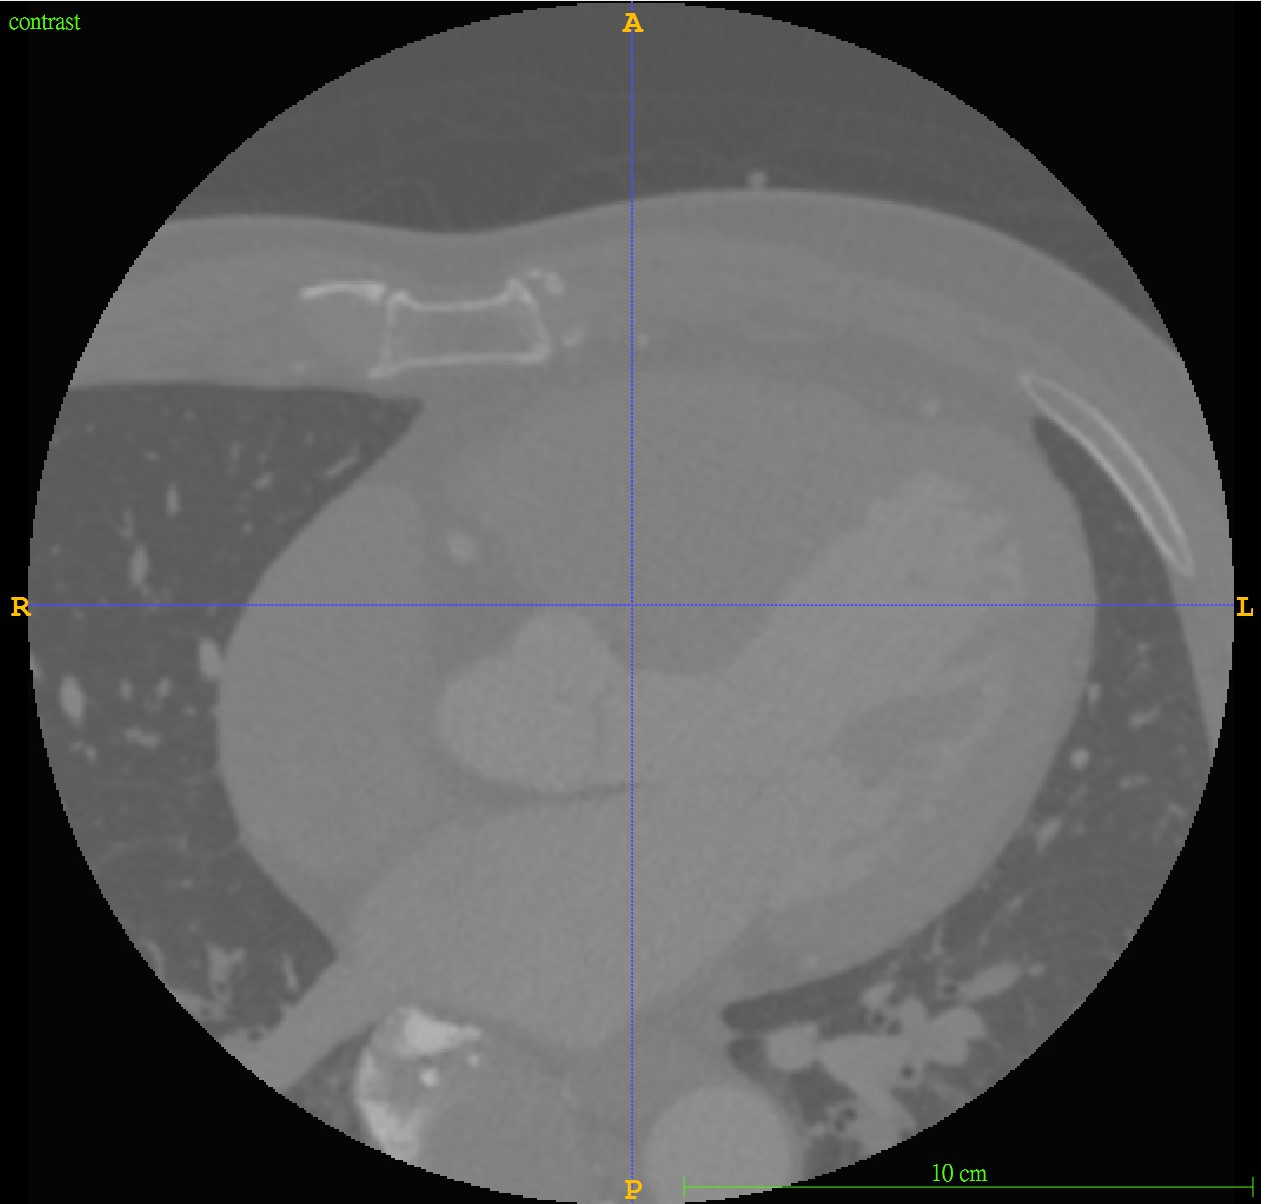
\includegraphics[width=0.4\linewidth]{fig-dataset-contrast-origin}}
    ~
    \subcaptionbox
        {調整後
        \label{fig:fig-dataset-contrast-after-adjustment}}
        {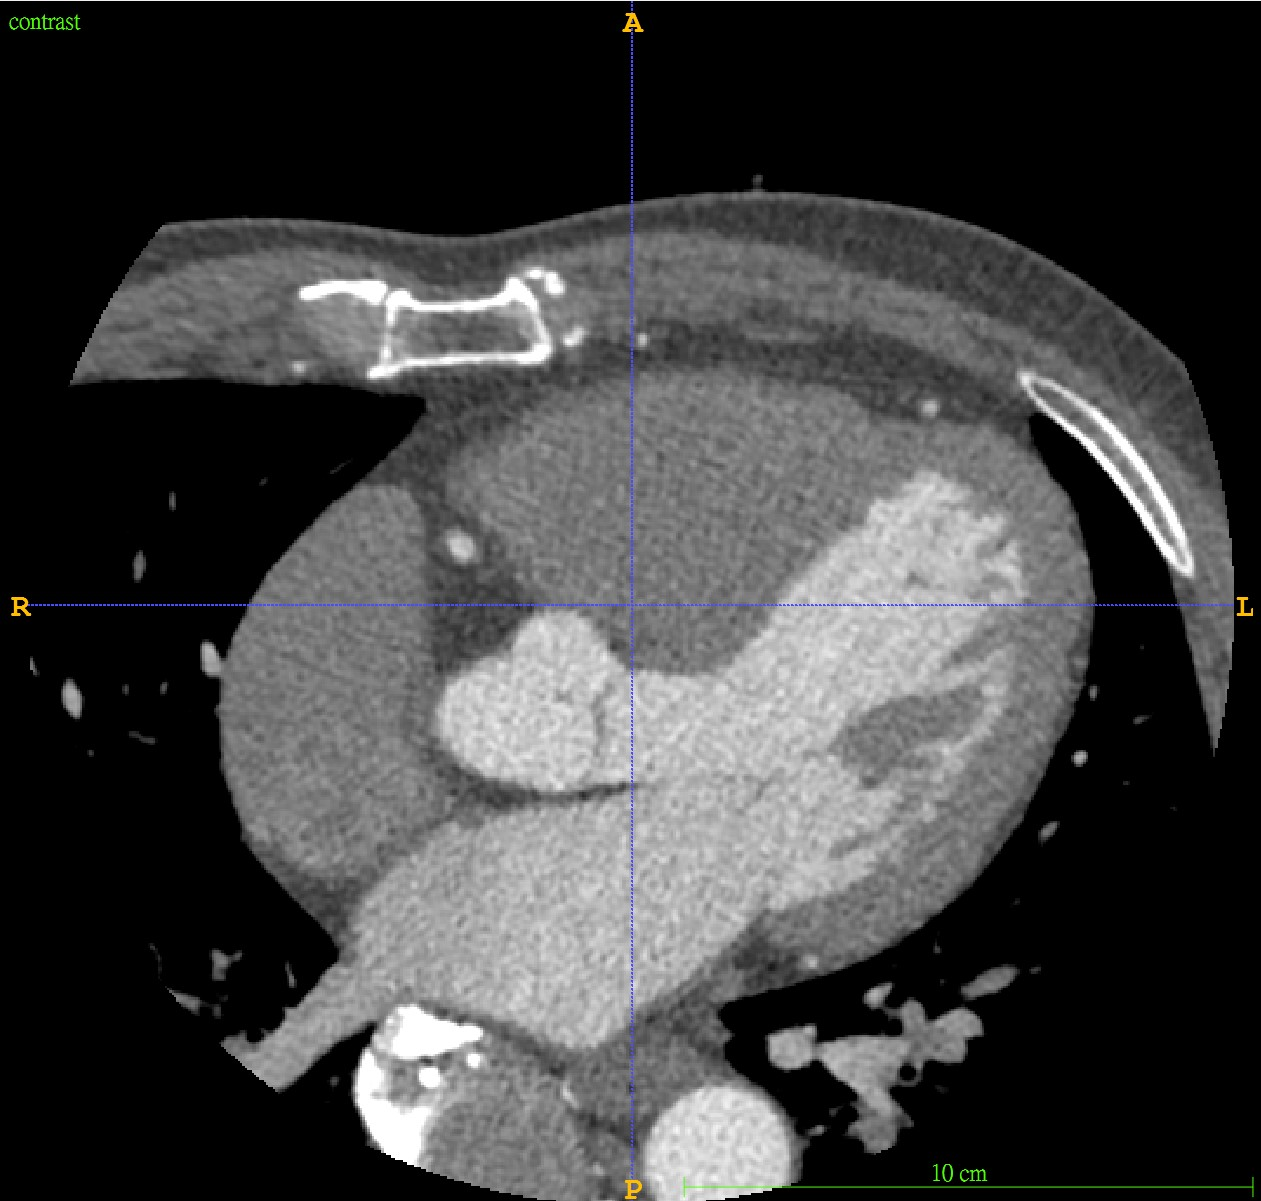
\includegraphics[width=0.4\linewidth]{fig-dataset-contrast-after-adjustment}}
    \caption{有顯影劑增強之電腦斷層影像數值調整}
    \label{fig:fig-dataset-contrast-before-after-adjustment}
\end{figure}

對於無顯影劑增強之電腦斷層影像也依照上述方式,以下界-300 HU以及上界500 HU進行調整。
\cref{fig:fig-dataset-cs-before-after-adjustment}為調整前後之影像以灰階圖呈現的結果。

\begin{figure}[!hbt]
    %\captionsetup[subfigure]{labelformat=empty} % 完全隱藏圖號
    \centering
    \subcaptionbox
        {調整前
        \label{fig:fig-sample-cs-before-adjustment}}
        {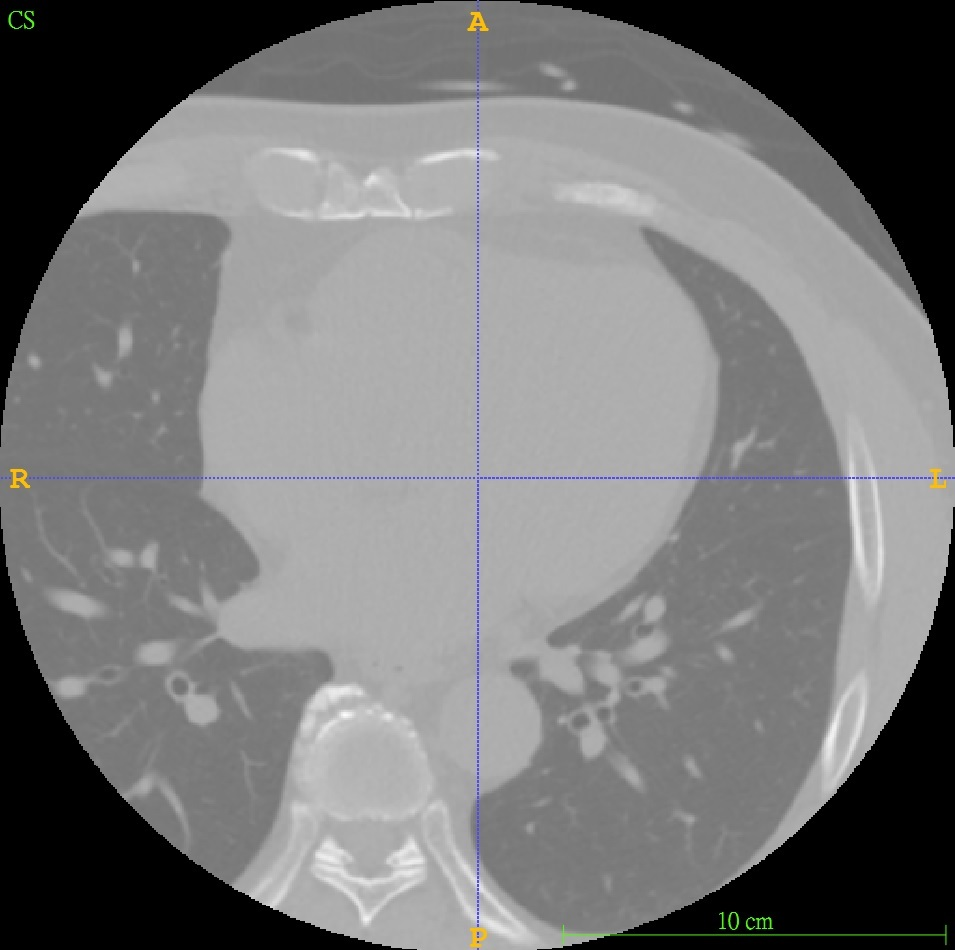
\includegraphics[width=0.4\linewidth]{fig-sample-cs-before-adjustment.jpg}}
    ~
    \subcaptionbox
        {調整後
        \label{fig:fig-sample-cs-after-adjustment}}
        {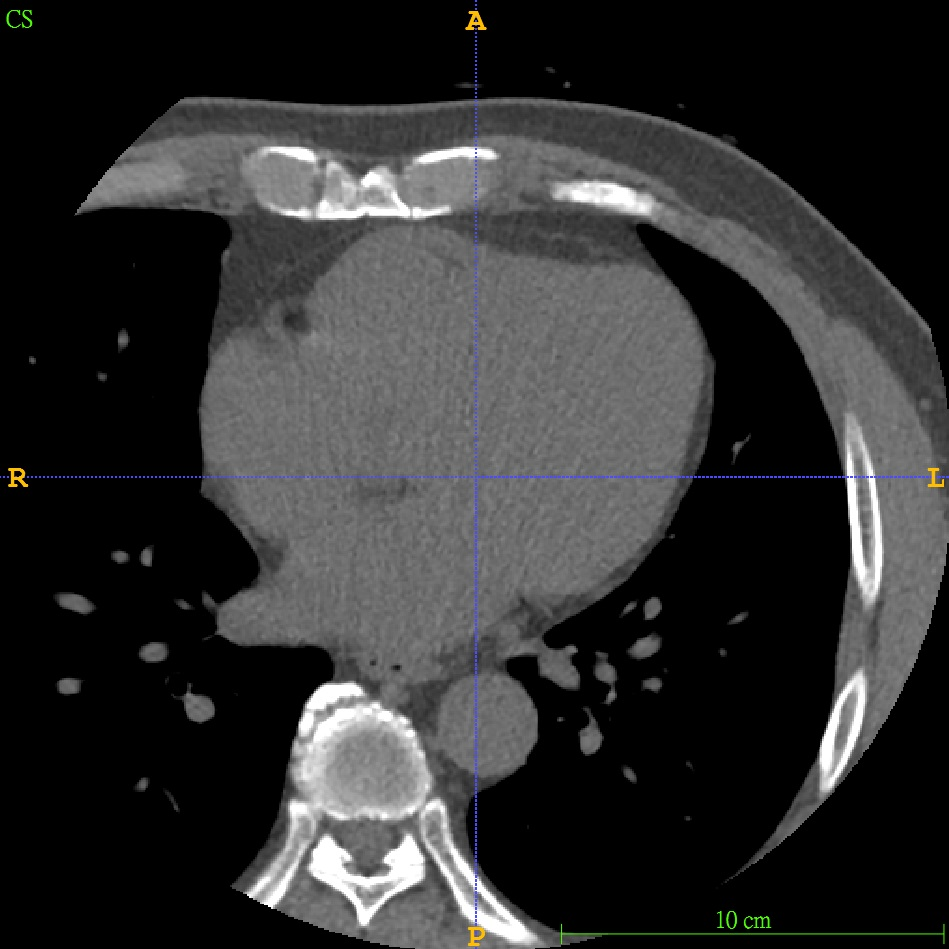
\includegraphics[width=0.4\linewidth]{fig-sample-cs-after-adjustment.jpg}}
    \caption{無顯影劑增強之電腦斷層影像數值調整}
    \label{fig:fig-dataset-cs-before-after-adjustment}
\end{figure}

\subsection{影像壓縮}
由於原始影像大小過於龐大,受限於運算資源,無法一次使用完整的3D影像進行訓練,
因此影像在輸入模型進行訓練、預測前會先進行圖片大小壓縮,
並將模型輸出結果以線性內插轉換回原始大小進行評估。
\cref{table:table-image-size-compress}為原始影像大小以及壓縮後的大小,
\cref{table:table-image-size-compress}中的數值分別為三維影像之長、寬、高像素數量。
\begin{table}[h]
    \centering
    \caption{原始影像大小及壓縮後大小}
    \label{table:table-image-size-compress}
    \begin{tabular}{|c|c|c|}
    \hline
    名稱 & 原始影像大小 & 壓縮後大小 \\
    \hline
    有顯影劑增強影像 & (512, 512, 256) & (192, 192, 192) \\
    \hline
    無顯影劑增強影像 & (512, 512, 64) & (256, 256, 64) \\
    \hline
    \end{tabular}
\end{table}

\section{無顯影劑影像資料擴增模型}
\cref{fig:fig-sample-with-without-contrast}為自同一受檢者拍攝之有、無顯影劑之電腦斷層影像,
從資料中可以觀察到無顯影劑增強之電腦斷層影像對於血管對比度較低,在有顯影劑增強之電腦斷層影像,如\cref{fig:fig-sample-contrast}中,心臟血液流經的部分為白色,與其他組織較有差異性;
而在無顯影劑增強之電腦斷層影像,如\cref{fig:fig-sample-cs}中,心臟血液流經的部分則與其他組織較無差異。
\begin{figure}[!hbt]
    %\captionsetup[subfigure]{labelformat=empty} % 完全隱藏圖號
    \centering
    \subcaptionbox
        {有注射顯影劑
        \label{fig:fig-sample-contrast}}
        {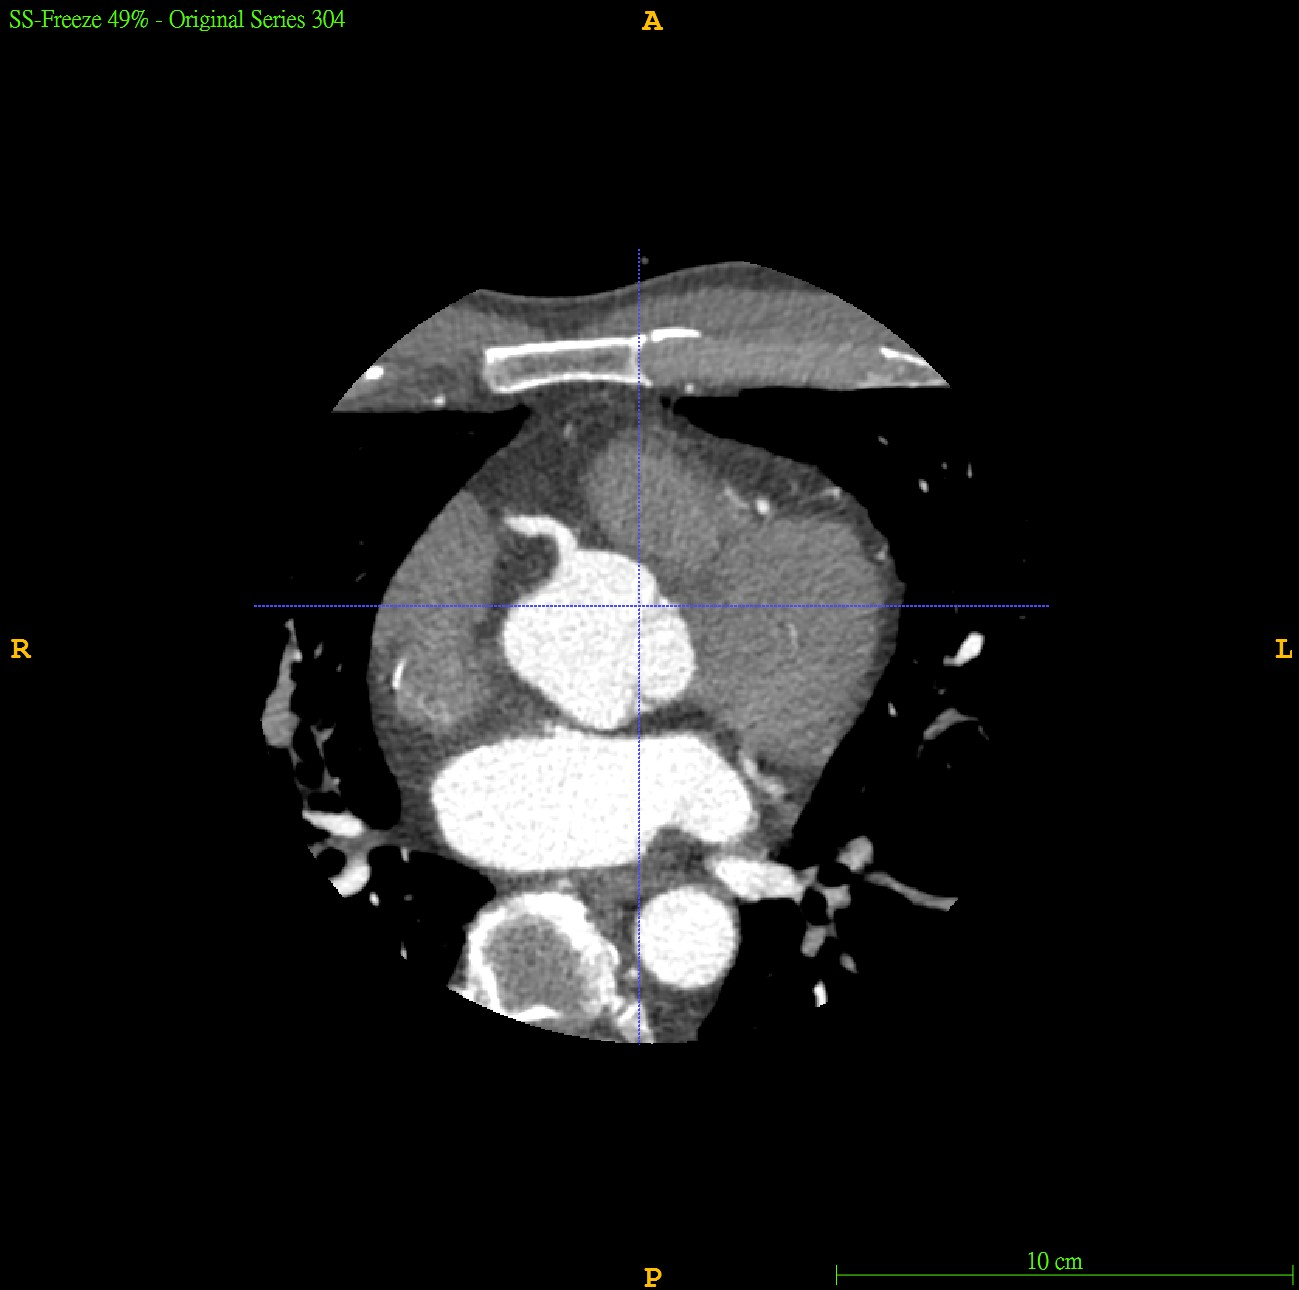
\includegraphics[width=0.475\linewidth]{fig-sample-contrast.jpg}}
    ~
    \subcaptionbox
        {無注射顯影劑
        \label{fig:fig-sample-cs}}
        {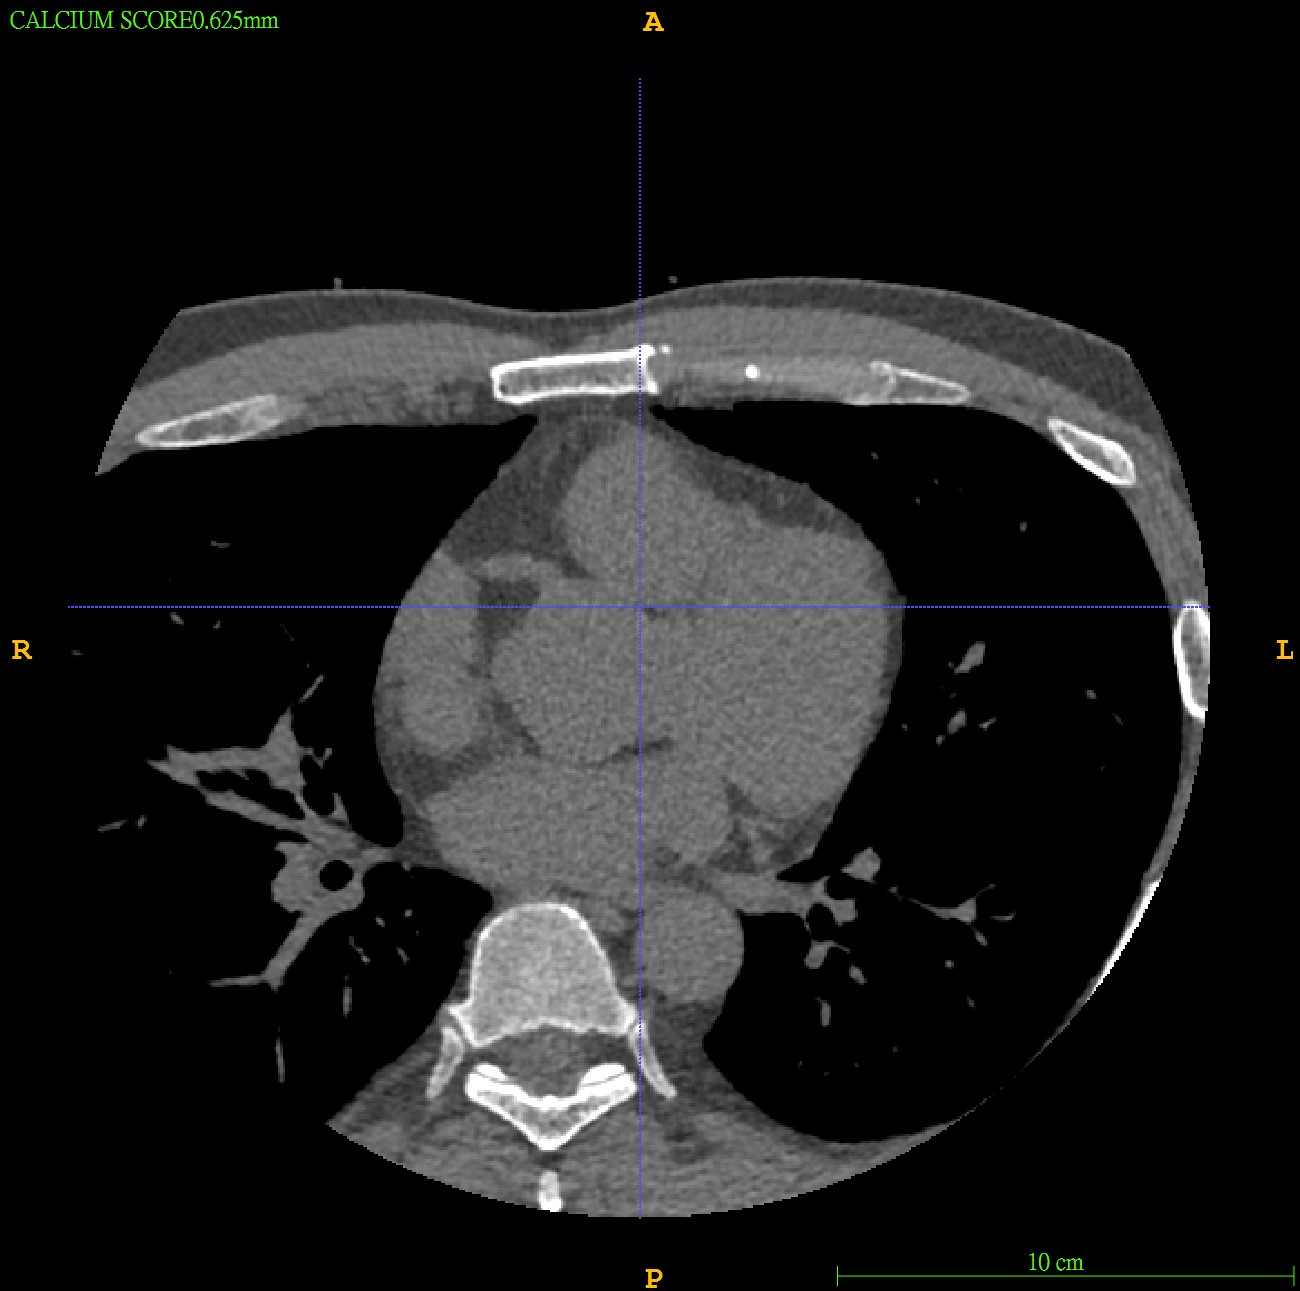
\includegraphics[width=0.475\linewidth]{fig-sample-cs.jpg}}
    \caption{有無顯影劑增強之電腦斷層影像}
    \label{fig:fig-sample-with-without-contrast}
\end{figure}

此種差異增加了標記資料的難度,使得原本就需要耗費大量時間的人工標記血管任務,
在無顯影劑增強的電腦斷層影像中更為困難,
且標記之血管結果不如血管對比度較高的有顯影劑增強之電腦斷層影像,
使得取得品質優良之標記資料難度也更高。

一個能利用既有資料輔助訓練的想法是,
將已標記之有顯影劑增強之電腦斷層掃描影像進行影像風格轉換,
將其轉換為無顯影劑增強之電腦斷層掃描影像做為額外的訓練資料。
其中CycleGAN已被許多研究用於醫學影像之影像風格轉換研究
~\cite{jiangTumorAwareAdversarialDomain2018, welanderGenerativeAdversarialNetworks2018, songNoncontrastCTLiver2020},
目前也有研究使用深度學習技術進行醫學影像的轉換,並用於資料擴增的任務上~\cite{songNoncontrastCTLiver2020}。

本研究使用CycleGAN訓練一個影像風格轉換模型,
將有顯影劑增強之電腦斷層影像轉換為虛擬的無顯影劑增強之電腦斷層影像,
即是將\cref{fig:fig-sample-contrast}轉換為\cref{fig:fig-sample-cs},
並使用在有顯影劑增強之電腦斷層影像標註之冠狀動脈分割標記,
做為無顯影劑增強之電腦斷層影像冠狀動脈分割任務的擴充資料,
期望能以現有資料增加分割模型的效果。

有無使用CycleGAN對於訓練無顯影劑增強之電腦斷層影像冠狀動脈分割模型的結果,
會在實驗設計與結果的章節進行討論。

\section{冠狀動脈分割}
目前已有許多研究
~\cite{huangCoronaryArterySegmentation2018, chenCoronaryArterySegmentation2019}
對於有顯影劑增強之電腦斷層影像進行冠狀動脈分割的任務達成不錯的成果,
3D U-Net是其中被廣泛運用於醫學影像分割的模型,因此本研究使用3D U-Net做為冠狀動脈分割任務之模型。

模型訓練所使用的目標函數為骰子損失函數(Dice Loss),其函式為\cref{eqn:dice-loss}
\begin{equation}
\label{eqn:dice-loss}
Loss = 1-\frac{2|X\cap Y|}{|X|+|Y|} 
\end{equation}
其中X、Y分別為模型預測結果以及模型預期結果,
當兩者重疊部分越多且不重疊部分越少時,損失數值越低,反之則愈高。

雖然有顯影劑增強之電腦斷層影像相較於無顯影劑增強之電腦斷層影像能夠更精確地顯示血管位置,
並取得較佳的冠狀動脈分割結果,然而部分對於碘成分過敏或是腎臟功能有問題的受檢者,
可能會對顯影劑產生不良反應
~\cite{andreucciUpdateRenalToxicity2017,rasuliMetforminContrastMedia1998,saljoughianIntravenousRadiocontrastMedia2012},
這些受檢者較不適合使用顯影劑,
因此本研究也實驗了以無顯影劑增強之電腦斷層影像進行冠狀動脈分割實驗,
期望提供不適合注射顯影劑的受檢者初步的冠狀動脈分割,
以輔助醫師在後續的診斷流程。


\section{有顯影劑冠狀動脈分割之相關應用}
\subsection{鈣化位置偵測}
目前在進行完整的冠狀動脈疾病風險評估時,
會需要同時使用有顯影劑以及無顯影劑增強之影像,
分別進行冠狀動脈分割以及鈣化位置偵測,
流程如\cref{fig:fig-contrast-cs-ct-examination}所示,
在進行電腦斷層掃描攝影時,
受檢者會先在無注射顯影劑時進行電腦斷層影像攝影,
取得無顯影劑增強之電腦斷層影像,接著再接受顯影劑注射,
進行第二次電腦斷層影像攝影取得有顯影劑增強之電腦斷層影像。

\fig[0.2][fig:fig-contrast-cs-ct-examination][!hbt]{fig-contrast-cs-ct-examination.jpg}[冠狀動脈疾病風險評估流程][冠狀動脈疾病風險評估流程]

有顯影劑增強之影像將會利用於標註冠狀動脈結構,
使得醫師能夠了解受檢者的冠狀動脈結構、是否有血管狹窄度的情形,
無顯影劑增強之影像則會利用於鈣化位置標註,
使得醫師能夠了解受檢者的冠狀動脈是否有鈣化以及鈣化的位置,
將冠狀動脈結構以及鈣化位置搭配進行參考,
能夠更精確地了解鈣化在血管中的位置。

然而在這樣的流程下,受檢者會需要接受兩次的電腦斷層影像攝影,
接受兩次的輻射暴露,
因此本研究希望能直接使用有顯影劑增強之電腦斷層影像進行鈣化位置評估,
透過提供醫生輸入欲擷取之HU值閥值,
利用血管分割模型的結果擷取出血管周遭的鈣化位置並以視覺化呈現,
使得受檢者只需進行一次有注射顯影劑之電腦斷層掃描攝影,
便能找到其血管中可能有鈣化的位置,
降低受到輻射暴露的風險。

\fig[0.2][fig:fig-contrast-calcium-location][!hbt]{fig-contrast-calcium-location.jpg}[僅以有顯影劑資料進行鈣化位置偵測流程][僅以有顯影劑資料進行鈣化位置偵測流程]

本研究的流程如\cref{fig:fig-contrast-calcium-location}所示,
受檢者會在注射顯影劑後進行電腦斷層掃描攝影,
透過本研究提出之冠狀動脈分割模型進行自動冠狀動脈分割,
並使用冠狀動脈分割結果、原始電腦斷層影像、以及使用者輸入之目標HU閥值,
透過取三者之交集,將血管位置中超過使用者輸入HU閥值之位置視為鈣化位置,
並將其以視覺化呈現,提供醫生進行診斷時參考。


\subsection{狹窄度分析}
在冠狀動脈心臟病的診斷中,血管狹窄度是一個重要的指標,
目前醫師可以透過電腦斷層掃描影像或分割之血管結果,
了解受檢者之血管管徑趨勢,藉以診斷受檢者是否有血管狹窄的情形。

然而單純以目視的方式難以精準的了解受檢者之血管管徑數據,
且冠狀動脈是一個在三維空間中往不同方向發展的結構,
在判斷血管管徑時會需要考慮到不同觀察方向,
也使得進行診斷時的不便,
因此本研究期望能提供醫師於血管狹窄度分析時更方便的資料,
藉由冠狀動脈分割結果取得其中心線,
將原始影像轉換為以中心線投影之拉直後之影像,
使得更容易的看出血管管徑趨勢,
此外,本研究也以拉直後之影像計算血管管徑並繪製成趨勢圖,
以方便醫師進行對血管狹窄度的分析。

\fig[0.25][fig:fig-stenosis-detection][!hbt]{fig-stenosis-detection.jpg}[狹窄度分析流程][狹窄度分析流程]

\begin{figure}[!hbt]
    %\captionsetup[subfigure]{labelformat=empty} % 完全隱藏圖號
    \centering
    \subcaptionbox
        {原始分割結果
        \label{fig:fig-before-skeleton}}
        {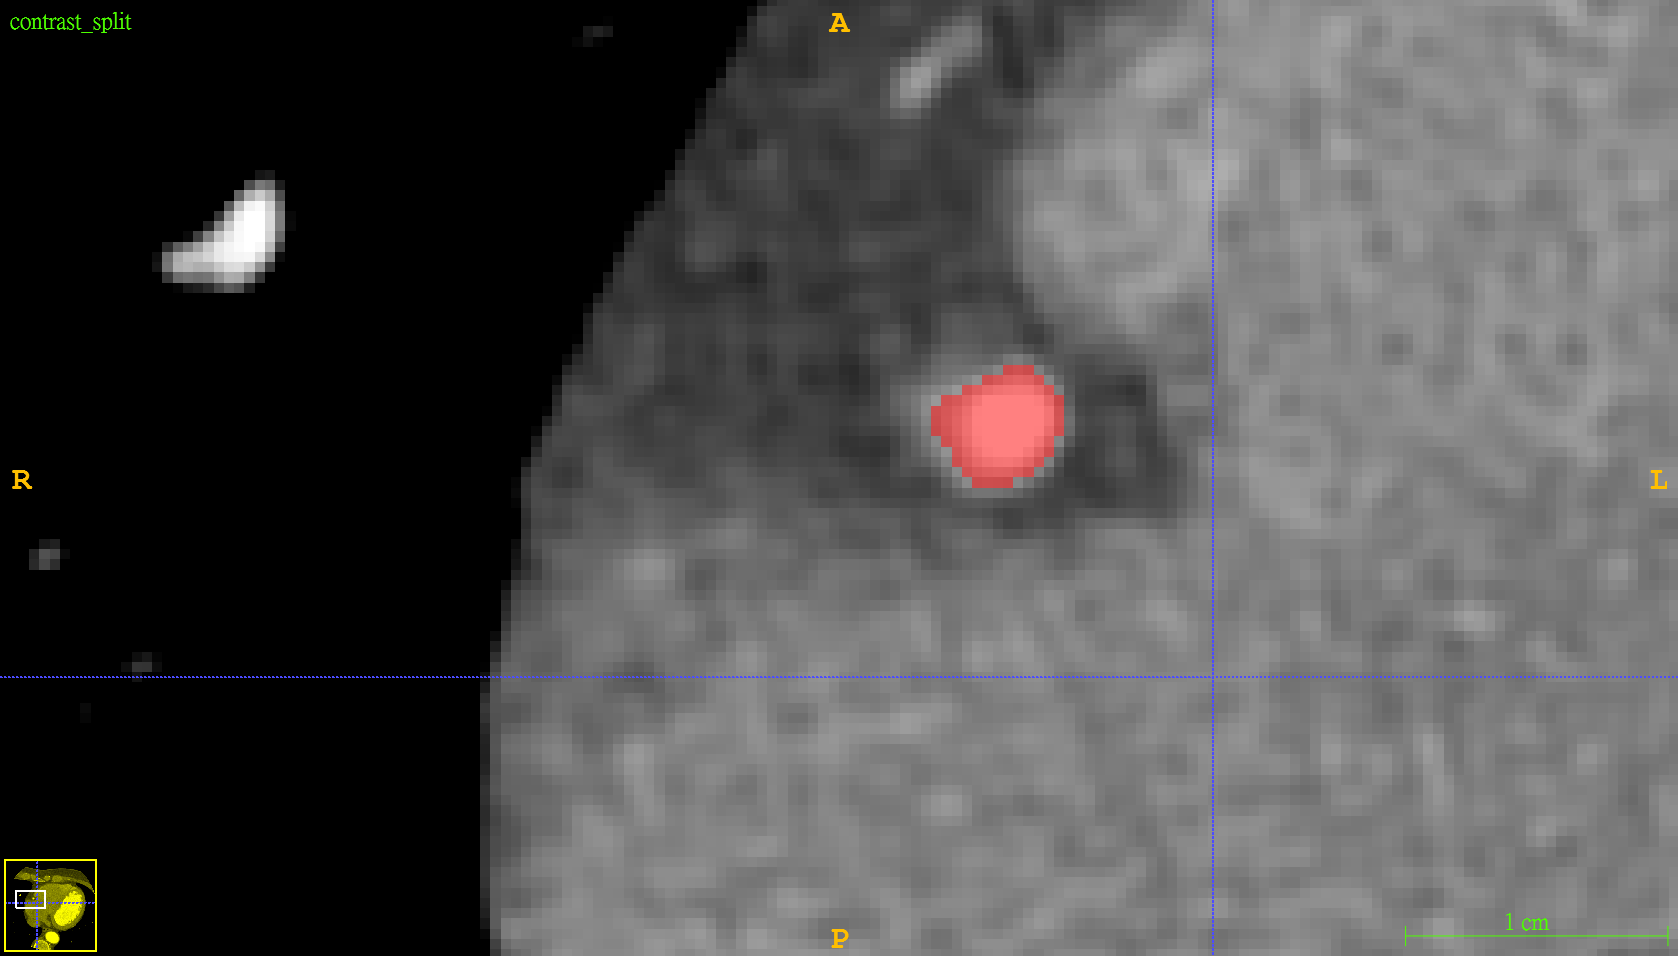
\includegraphics[width=0.475\linewidth]{fig-before-skeleton.jpg}}
    ~
    \subcaptionbox
        {細線化之結果
        \label{fig:fig-after-skeleton}}
        {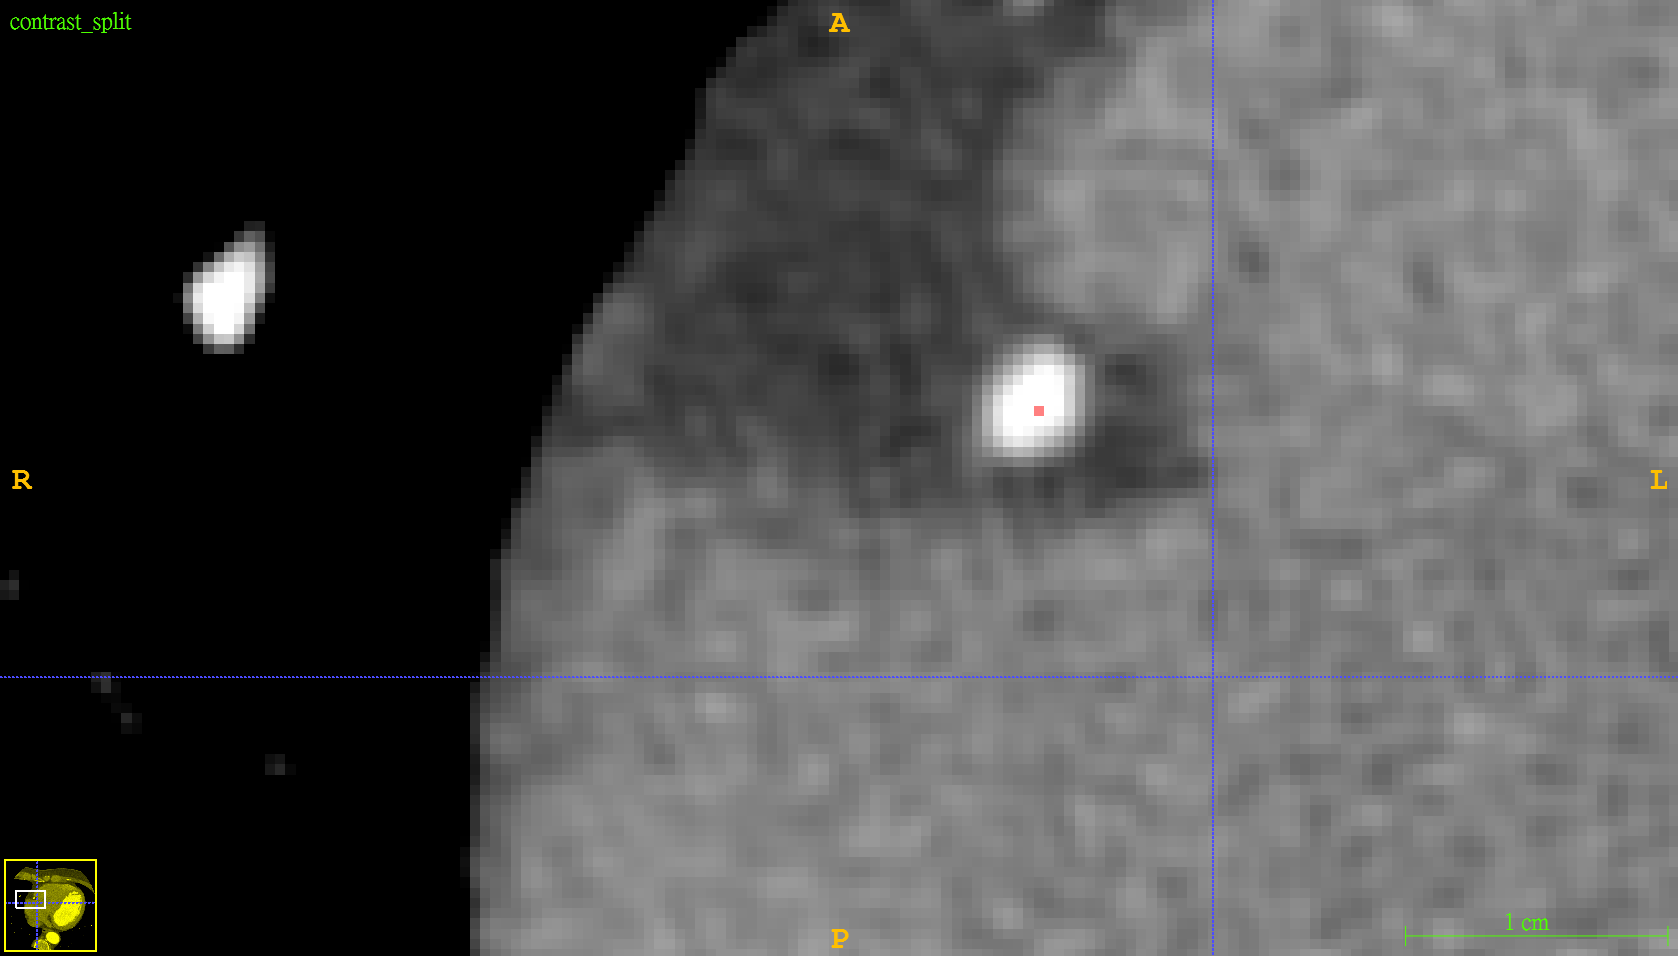
\includegraphics[width=0.475\linewidth]{fig-after-skeleton.jpg}}
    \caption{細線化處理取得中心線}
    \label{fig:fig-skeleton}
\end{figure}

\fig[0.75][fig:fig-cpr-y][!hbt]{fig-cpr-y.jpg}[以血管中心線拉直之原始影像][以血管中心線拉直之原始影像]

\begin{figure}[!hbt]
    %\captionsetup[subfigure]{labelformat=empty} % 完全隱藏圖號
    \centering
    \subcaptionbox
        {原始分割結果
        \label{fig:fig-before-cpr}}
        {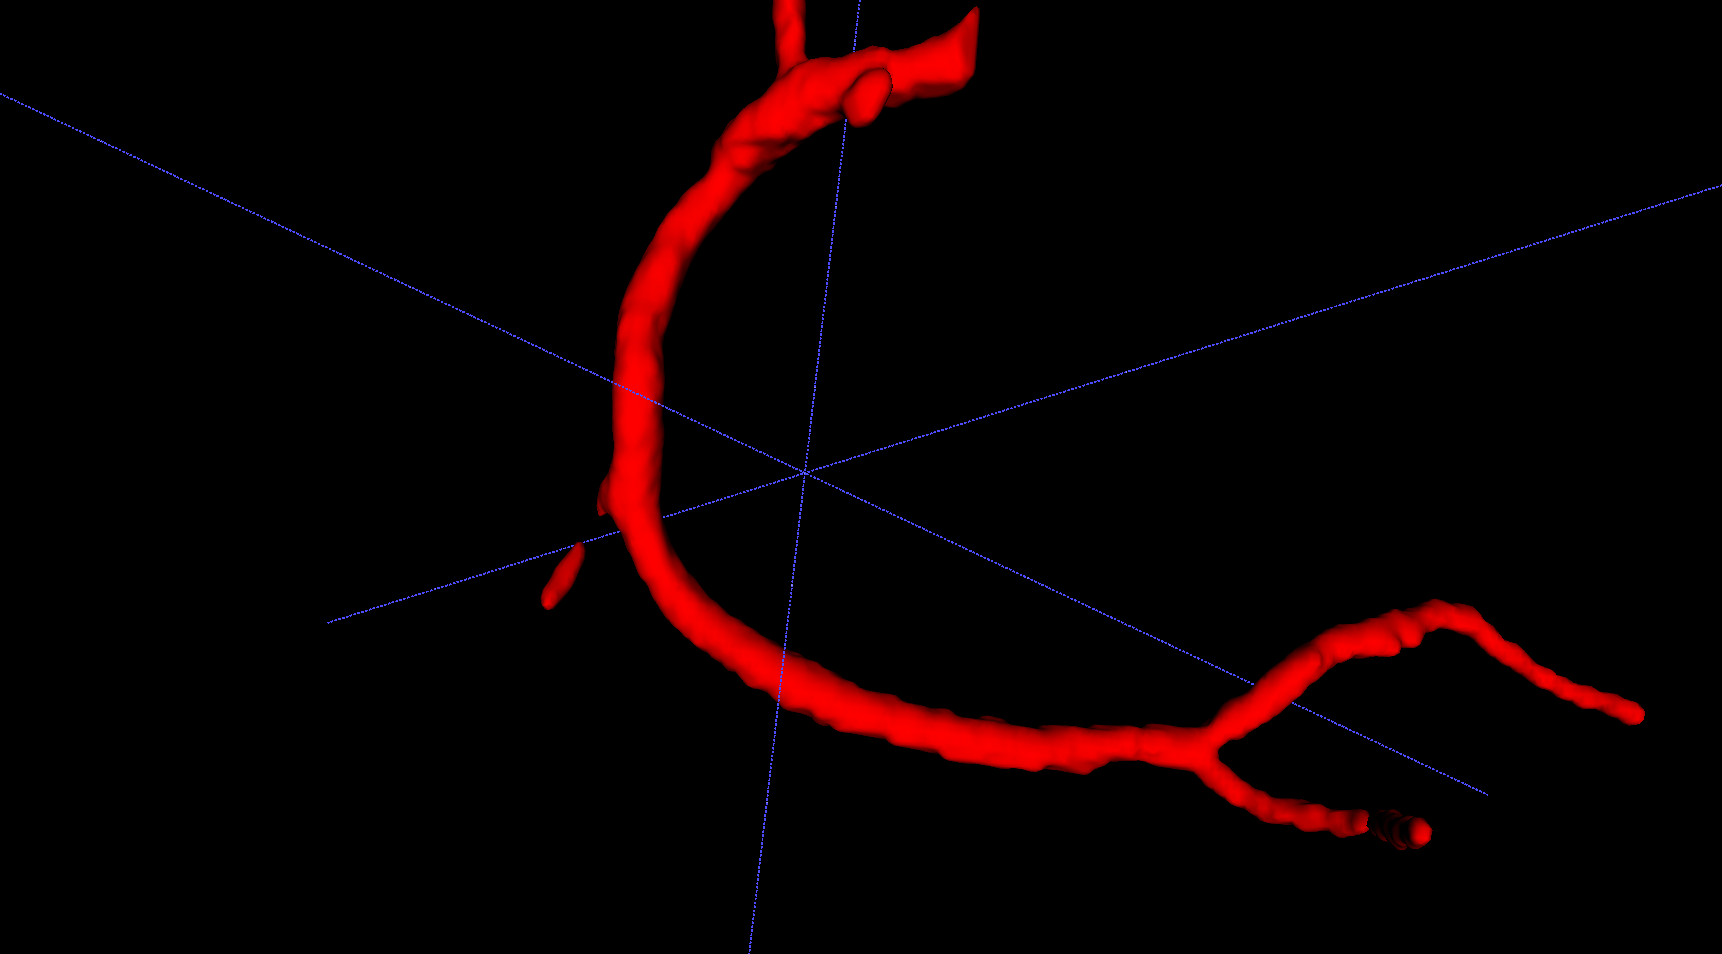
\includegraphics[width=0.475\linewidth]{fig-before-cpr.jpg}}
    ~
    \subcaptionbox
        {利用中心線拉直之結果
        \label{fig:fig-after-cpr}}
        {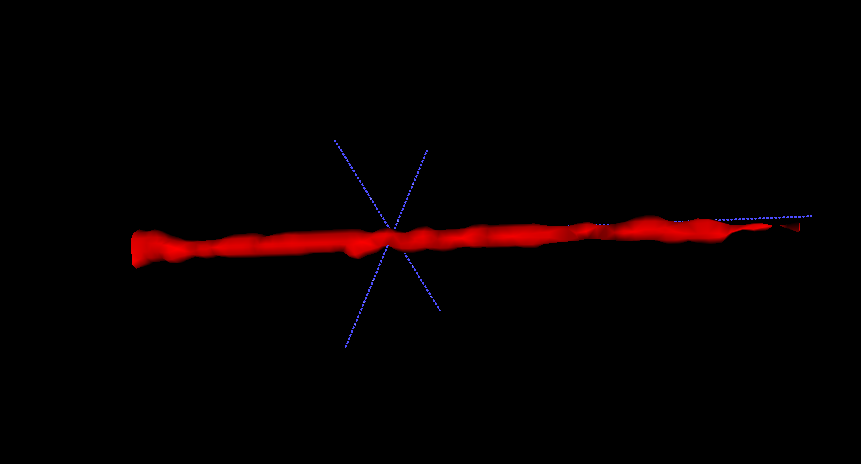
\includegraphics[width=0.475\linewidth]{fig-after-cpr.jpg}}
    \caption{以血管中心線拉直之冠狀動脈分割}
    \label{fig:fig-cpr}
\end{figure}

本研究之狹窄度分析流程如\cref{fig:fig-stenosis-detection}所示,
首先會透過原始影像中分割出冠狀動脈結構,
並將分割結果進行細線化處理取得中心線,
中心線轉換的結果如\cref{fig:fig-skeleton},
\cref{fig:fig-skeleton}中紅色部分分別為原始分割結果以及細線化得到之中心線,
接著利用Curved Planar Reformation方法~\cite{kanitsarCPRCurvedPlanar2002}以血管中心線對原始影像進行座標轉換,
為利用血管中心線做為向量,產生以中心線之拉直後之影像,
原始影像以RCA主支中心線進行轉換的結果如\cref{fig:fig-cpr-y},
\cref{fig:fig-cpr-y}之結果會用提供給使用者做為額外的參考資料,
\cref{fig:fig-cpr}冠狀動脈分割以RCA主支中心線進行轉換的結果,
本研究會利用轉換後之冠狀動脈分割計算血管管徑,
並繪製成趨勢圖,以方便醫師進行對血管狹窄度的分析。


\subsection{資料視覺化}
本研究使用開源軟體3D Slicer
~\cite{theslicercommunity3DSlicerImage,fedorov3DSlicerImage2012,geringIntegratedVisualizationSystem1999,geringIntegratedVisualizationSystem2001,kapurIncreasingImpactMedical2016,kikinis3DSlicerPlatform2014,pieperNAMICKitITK2006}
做為資料視覺化平台,軟體介面如\cref{fig:fig-3dslicer-ul-example}。
\fig[0.75][fig:fig-3dslicer-ul-example][!hbt]{fig-3dslicer-ul-example.jpg}[3D Slicer軟體介面][3D Slicer軟體介面]

\fig[0.5][fig:fig-3dslicer-custom-extension-example][!hbt]{fig-3dslicer-custom-extension-example.jpg}[3D Slicer自定義套件][3D Slicer自定義套件]

3D Slicer提供多平台的桌面應用程式,
能在Windows, Linux, MacOS上運行,
並且支援多種格式的醫學影像資料、資料檢視方式以及資料處理工具,
此外,使用者能夠利用Python撰寫自定義的3D Slicer套件,
使得使用者能在3D Slicer中呼叫自行撰寫的Python程式、深度學習模型進行資料處理,
並將結果回傳至3D Slicer進行呈現。

本研究將冠狀動脈分割模型、鈣化位置分析模組、狹窄度分析模組以3D Slicer套件的形式整合至3D Slicer中,
套件介面如\cref{fig:fig-3dslicer-custom-extension-example},
使用者可以將心臟電腦斷層影像匯入至3D Slicer,
選取來源影像、是否有顯影劑以及HU範圍呼叫深度學習模型進行冠狀動脈自動標記。
對於有顯影劑影像所擷取出之冠狀動脈,可以設定HU閥值呼叫鈣化位置分析模組進行鈣化位置偵測,
此外,使用者能夠選取血管的兩端點呼叫狹窄度分析模組,
取得以中心線拉直後血管影像以及血管管徑趨勢圖。

\end{document}          % 研究方法
        \documentclass[class=NCU_thesis, crop=false]{standalone}
\begin{document}

\chapter{實驗設計與結果}

\section{嬰兒臉部偵測實驗}
\subsection{實驗目的與設計}
在收集嬰兒臉部資料集時,
需針對嬰兒影像擷取出臉部範圍,
進而後續之臉部遮擋辨識階段。

因此,本實驗使用3.3節之嬰兒姿勢資料集,
就OpenCV~\cite{goyal_face_2017}
、SSD~\cite{ye_face_2021}
、MTCNN~\cite{xiang_joint_2017}
及RetinaFace~\cite{deng_retinaface_2020}
等臉部偵測演算法,
分析其執行時間及臉部擷取準確度進行比較,
以驗證適合本系統之演算法。

\subsection{實驗評估方式}
本實驗為驗證嬰兒臉部偵測演算法之實際可行性,
將針對臉部偵測執行時間及偵測結果之準確度分別進行比較:
透過計算演算法偵測所有資料集共15416張影像所花費之時間,
得以算出各演算法平均每張需花費之時間;
而準確度則將嬰兒臉部偵測之影像結果進行分類標註,
分別計算出各演算法之accuracy、precision及recall。

\subsection{實驗結果與分析}
首先,針對演算法之執行時間進行比較,
透過實驗結果可得出使用SSD演算法進行嬰兒臉部偵測,
將可擁有較佳的偵測速度。
而四項演算法偵測15416張影像之詳細實驗結果如下:

(1)OpenCV演算法:
共花費18分01.78秒,
平均每張影像需花0.07秒;

(2)SSD演算法:
共花費9分17.26秒,
平均每張影像需花0.04秒;

(3)MTCNN演算法:
共花費2小時8分22.05秒,
平均每張影像需花0.50秒;

(4)RetinaFace演算法:
共花費XX,
平均每張影像需花XX秒。

接著,就偵測之精確度進行比較,
透過實驗結果可得出選用RetinaFace演算法進行嬰兒臉部偵測,
可擁有較佳的偵測準確度。
而四項演算法進行嬰兒臉部偵測之詳細實驗結果如下:

(1)使用OpenCV演算法偵測結果如\cref{table:table-opencv},
由於偵測效果不佳,
將多數影像皆誤判為False(無臉),
故僅計算其precision為79.90\%;

(2)使用SSD演算法偵測結果如\cref{table:table-ssd},
由於偵測效果不佳,
將多數影像皆誤判為False(無臉),
故僅計算其precision為99.90\%;

(3)使用MTCNN演算法偵測結果如\cref{table:table-mtcnn},
其accuracy為90.20\%、precision為94.76\%以及recall為90.93\%;

(4)使用RetinaFace演算法偵測結果如\cref{table:table-retinaface},
其accuracy為99.78\%、precision為99.75\%以及recall為99.91\%。

綜觀上述兩部分實驗結果,
若系統欲擁有較迅速的執行速度又兼具偵測準確度,
可得出以下結論:
先使用SSD演算法找尋嬰兒臉部範圍,
雖然此方法在許多狀況未能如期找到嬰兒臉部範圍,
但其準確度很高,
故能利用此算法之時間優勢;
而若SSD演算法找不到嬰兒臉部時,
則接續使用RetinaFace演算法,
利用其很高之正確率及準確率之特質進行嬰兒臉部偵測。

\begin{table}[h]
    \centering
    \caption{OpenCV演算法偵測嬰兒臉部結果}
    \label{table:table-opencv}
    \begin{tabular}{ccc}
    \hline
     & True(預測有臉)& False(預測無臉)\\
    \hline
    True & \multirow{2}{*}{2882} & \multirow{4}{*}{11809} \\
    (實際有臉)& & \\
    False & \multirow{2}{*}{725} & \\
    (實際無臉)&  & \\
    \hline
    \end{tabular}
\end{table}

\begin{table}[h]
    \centering
    \caption{SSD演算法偵測嬰兒臉部結果}
    \label{table:table-ssd}
    \begin{tabular}{ccc}
    \hline
     & True(預測有臉)& False(預測無臉)\\
    \hline
    True & \multirow{2}{*}{4830} & \multirow{4}{*}{10581} \\
    (實際有臉)& & \\
    False & \multirow{2}{*}{5} & \\
    (實際無臉)&  & \\
    \hline
    \end{tabular}
\end{table}

\begin{table}[h]
    \centering
    \caption{MTCNN演算法偵測嬰兒臉部結果}
    \label{table:table-mtcnn}
    \begin{tabular}{ccc}
    \hline
     & True(預測有臉)& False(預測無臉)\\
    \hline
    True & \multirow{2}{*}{9361} & \multirow{2}{*}{994} \\
    (實際有臉)& & \\
    False & \multirow{2}{*}{517} & \multirow{2}{*}{4544} \\
    (實際無臉)&  & \\
    \hline
    Total & \textbf{9878} & \textbf{5538} \\
    \hline
    \end{tabular}
\end{table}

\begin{table}[h]
    \centering
    \caption{RetinaFace演算法偵測嬰兒臉部結果}
    \label{table:table-retinaface}
    \begin{tabular}{ccc}
    \hline
     & True(預測有臉)& False(預測無臉)\\
    \hline
    True & \multirow{2}{*}{12925} & \multirow{2}{*}{11} \\
    (實際有臉)& & \\
    False & \multirow{2}{*}{33} & \multirow{2}{*}{2447} \\
    (實際無臉)&  & \\
    \hline
    Total & \textbf{12958} & \textbf{2458} \\
    \hline
    \end{tabular}
\end{table}

\section{臉部遮擋辨識實驗}
\subsection{模型訓練結果}
準確率達98\%,
詳細訓練結果請見\cref{fig:fig-result-face}。
\fig[0.8][fig:fig-result-face][!hbt]{fig-result-face.png}[臉部辨識訓練結果][臉部辨識訓練結果]

\subsection{實驗設計}
使用ResNet50~\cite{he_deep_2016}
訓練臉部遮擋模型與奶嘴辨識模型,
訓練回合數皆為20。

\subsection{實驗評估方式}
奶嘴辨識實驗實驗評估方式 奶嘴辨識實驗實驗評估方式

\subsection{實驗結果分析}
首先,使用503張影像測試臉部遮擋辨識,
其中僅一張影像(
\cref{fig:fig-face-pacifier-error}。
\fig[0.4][fig:fig-face-pacifier-error][!hbt]{fig-face-pacifier-error.jpg}[誤判影像:真實類別為安全,但預測為警示][誤判影像:真實類別為安全,但預測為警示]
)類別判斷錯誤,
誤將安全狀態辨識為警示狀態。
推測原因為該張影像畫質較差,面部影像不清而導致誤判。

再者,我們使用232張影像測試奶嘴辨識,
所有測試集皆辨識正確。

由於此二模型測試正確率高,故本文中不放入其混淆矩陣。

\section{姿勢分類實驗}
\subsection{模型訓練結果}
準確率達99\%,
詳細訓練結果請見\cref{fig:fig-result-four-classes}。
\fig[0.8][fig:fig-result-four-classes][!hbt]{fig-result-four-classes.png}[姿勢辨識訓練結果][姿勢辨識訓練結果]

\subsection{實驗設計}
使用ResNet50~\cite{he_deep_2016}
訓練臉部遮擋模型與奶嘴辨識模型,
訓練回合數皆為20。

\subsection{實驗評估方式}
姿勢分類實驗評估方式 姿勢分類實驗評估方式

\subsection{實驗結果分析}
我們使用744張影像針對此模型進行測試,
包含了五張類別辨識錯誤的影像,
其中有三張將坐姿誤判為趴躺姿勢,
推測原因為嬰兒雖呈現坐姿,
但上半身貼近其腿部,而導致誤判。

此模型之混淆矩陣,請見\cref{fig:fig-confusion-matrix-four-classes}。
\fig[1.1][fig:fig-confusion-matrix-four-classes][!hbt]{fig-confusion-matrix-four-classes.png}[嬰兒姿勢辨識之混淆矩陣][嬰兒姿勢辨識之混淆矩陣]

\section{影片危險偵測實驗}
\subsection{實驗設計}
影片危險偵測實驗 影片危險偵測實驗

\subsection{實驗評估方式}
影片危險偵測實驗 影片危險偵測實驗

\subsection{實驗結果分析}
影片危險偵測實驗 影片危險偵測實驗

\end{document}          % 實驗設計與結果
        \documentclass[class=NCU_thesis, crop=false]{standalone}
\begin{document}

\chapter{結論與未來展望}
本章節中,
對本論文進行總結,
並闡述本研究未來可發展與應用之處,
將透過以下兩章子節進行分述:
結論、未來展望。

\section{結論}
本論文基於深度學習技術,
透過嬰兒影像畫面進行危險偵測,
目前可進行兩大部分之偵測:
(1)嬰兒臉部遮擋辨識、及(2)嬰兒姿勢辨識,
其訓練及測試準確率皆達98\%以上。

本系統優於過往感測器式偵測之功能單一性及不便性,
也不同於既有之影像式偵測僅關注嬰兒呼吸或單一動作之研究,
而提供了關注於嬰兒臉部及動作之危險監測系統,
將有助於協助照護者,
並降低嬰兒猝死症發生風險。

另外,
由於目前未有公開之嬰兒資料集,
故本論文使用之所有嬰兒影像,
皆收集自網路上實際嬰兒照片或影片擷取,
再經前處理及分類標示而成。

\newpage

\section{未來展望}
本論文中,
目前僅辨識四項嬰兒姿勢,
若在偵測姿勢時加入時間資訊,
預期得以判斷更多嬰兒行為,
如:翻身及爬行等動作,
即可監測更多危險情境;
而除辨識嬰兒臉部遭異物遮蔽外,
若加入偵測面部表情等其他資訊,
亦可更詳盡監測嬰兒狀態,
以提醒照護者;
此外,
亦可提供多嬰兒情境之危險偵測,
則使用場景將可更廣泛。

而系統實作方面,
未來可提供設定觀測之年齡區間,
即可針對不同之特定年齡嬰幼兒警示其具危險性之動作,
以達到更符合實際使用情境的危險偵測;
亦可結合通訊社群軟體等,
如:Line或Telegram等,
進行即時之推播訊息以通知照顧者。

\end{document}      % 結論
    %     \documentclass[class=NCU_thesis, crop=false]{standalone}
\usepackage{showexpl}

\begin{document}

\chapter{章名(章節示例)}
章內容內容內容內容內容 \\
內容內容內容

\section{節名}
節內容內容內容內容內容 \\
內容內容內容

\subsection{小節名}
內容內容內容 \\
內容內容內容

\subsubsection{小小節}
內容內容內容 \\
內容內容內容

\paragraph{段}
內容內容內容 \\
內容內容內容

\subparagraph{小段}
內容內容內容 \\
內容內容內容


\chapter{文字}
第一行。
仍是第一行。 \\
第二行。


\chapter{圖片}
\section{插入單一圖片}
\fig[0.15][fig:label_test][!hbt]{logo-Linux.png}[caption][short caption]

\section{插入多張圖片}
\begin{figure}[!hbt]
    %\captionsetup[subfigure]{labelformat=empty} % 完全隱藏圖號
    \centering
    \subcaptionbox
        {caption\_1
        \label{fig:subfig_fig1}}
        {
\includegraphics[width=0.3\linewidth]{fig1.png}}
    ~
    \subcaptionbox
        {caption\_2
        \label{fig:subfig_fig2}}
        {
\includegraphics[width=0.3\linewidth]{fig2.eps}}
    \vspace{\baselineskip} % 分隔上下列
    \subcaptionbox
        {caption\_3
        \label{fig:subfig_fig3}}
        {
\includegraphics[width=0.6\linewidth]{fig3.png}}
    \caption{caption, 使用 \subref{fig:subfig_fig2}取得子圖(Debian)編號 }
    \label{fig:label}
\end{figure}


\chapter{表格}
\section{一般表格}
\begin{table}[h]
    \centering
    \caption{Solution}
    \begin{tabular}{| l | l |}
        \hline
        Component & Concentration(mM) \\ \hline
        \ce{NaCl} & 118.0 \\ \hline
    \end{tabular}
\end{table}

\section{自動折行表格}
\begin{table}[h]
    \centering
    \begin{tabularx}{\textwidth}{| l | X |}
        \hline
        short & short short \\ \hline
        long & long long long long long long long long long long  long long long long long long long long long long\\ \hline
    \end{tabularx}
\end{table}

\end{document}
    \backmatter          % book class 預設\backmatter 在\appendix 後面。因此.cls修改過\appendix 定義
        % This file has 3 types bibliography management, 
% \bibManType in config.tex choose it.
% 0. Embedded: write \bibitem in {thebibliography} environment.
% 1. BibTeX: Change bib files in \bibliography{}
% 2. biber / BibLaTeX: Add bibliography by \addbibresource{bibfile.bib} in macros_preamble.tex

\documentclass[class=NCU_thesis, crop=false]{standalone}

\begin{document}

\ifcase \bibManType 
    % 0 == Embedded %%%%%%%%%%%%%%%%%%%%%%%%%%%%%%%%%%%%%%%
    {\bibFontStyle\setstretch{\bibLineStretch}
    \begin{thebibliography}{99}

    \bibitem{cite_key_1}
        bibliography item detail.

    \bibitem{_sppmg/tw_thesis_template_????}
        TW\_Thesis\_Template,
        sppmg,
        \url{https://github.com/sppmg/TW_Thesis_Template},
        Embedded bibliography demo.

    \end{thebibliography}
    }
    
\or
    % 1 == BibTeX %%%%%%%%%%%%%%%%%%%%%%%%%%%%%%%%%%%%%%%%%
    \bibliographystyle{\bibStyle}
    {\bibFontStyle\setstretch{\bibLineStretch}
        \bibliography{demo} % {sample_1,sample_2,...,sample_n}
        % Note the lack of whitespace between the commas and the next bib file.
    }
\or

    % 2 == biber / BibLaTeX %%%%%%%%%%%%%%%%%%%%%%%%%%%%%%%
    \printbibliography[title = {參考文獻}, heading = bibnumbered]
\fi



\end{document}
    % \appendix
    %     \documentclass[class=NCU_thesis, crop=false]{standalone}
\begin{document}

\chapter{裝置列表}

\begin{table}[!h]
    \centering
    \begin{tabularx}{\textwidth}{|l|l|X|}
        \hline
        裝置	     & 型號      & 說明 \\ \hline
        Linux    & Debian 9 & 世界好用的作業系統 \\ \hline
        Windows  & 10       & 防止人腦老化的工具 \\ \hline
    \end{tabularx}
    \caption{裝置列表}
    \label{table:list_device}
\end{table}

\end{document}
    %     \documentclass[class=NCU_thesis, crop=false]{standalone}
\begin{document}

\definecolor{Gray3}{gray}{0.8}

\chapter{Solutions}

\section{The solution}
\begin{table}[!h]
    \centering
    \begin{tabular}{| l | l |}
        \hline
        Component & Concentration(mM) \\ \hline
        \rowcolor{Gray3}
        \ce{NaCl} & 1.0 \\ \hline
        \ce{CaCl_2} & 2.0 \\ \hline
        \rowcolor{Gray3}
        \ce{NaCl} & 1.0 \\ \hline
        \ce{CaCl_2} & 2.0 \\ \hline
    \end{tabular}
    \caption{The solution}
\end{table}
\end{document}
    %     \documentclass[class=NCU_thesis, crop=false]{standalone}
\begin{document}
% Here demo instert whole code file. You can only insert code directly, 
% please read my tutorial or document of listings package.
% code style set in macros_preamble already.
% Supported language please read document of listings package or
% https://www.sharelatex.com/learn/Code_listing#!#Supported_languages

\chapter{程式碼}
\section{C}
\lstinputlisting[language=C]{hello_world_c.c}

\section{Matlab}
\lstinputlisting[language=matlab]{hello_world_matlab.m}

\section{IDL}
\lstinputlisting[language=IDL]{hello_world_idl.pro}
\end{document}

    %     \documentclass[class=NCU_thesis, crop=false]{standalone}

\begin{document}
\chapter{自動填單}
這裡試著幫各位自動填入部份資訊,其餘打勾、日期請手寫。有字體大小不符、位置歪掉等問題的話,請修改 appendix\_letter\_NCU.tex後直接編譯生成文件。

appendix\_letter\_NCU.tex中,每個句子(文字項目)都是獨立的大小與位置。 大小可由\textbackslash{}fs,調整。
\footnote{\textbackslash{}fs 使用 \textbackslash{}fontsize 做無級調整,並固定單行高度。 }
位置可由\textbackslash{}placetextbox 調整。語法如下:
\begin{lstlisting}[style=LatexStyle,caption={}]
\placetextbox{x(mm)}{y(mm)}
\end{lstlisting}
單位使用mm ,(0,0)位於左下角。建議調整時將``colorgrid''加入documentclass選項。(加入子檔的即可)
\begin{lstlisting}[style=LatexStyle,caption={}]
\documentclass[class=NCU_thesis, crop=false, colorgrid]{standalone}
\end{lstlisting}
colorgrid 將顯示格線(一小格是\SI{5}{\milli\metre})。

\begin{center}
{ \noindent\color{red}\bfseries\Large NCU English letters in the NCU\_en}
\end{center}

%%%%%%%%%%%%%%%%%%%%%%%%%%%%%%%%

% define \mprof 
\ExplSyntaxOn
    % Copy prof. list from config.tex
    \clist_gclear_new:N \g_sppmg_profs_cl
    \clist_gset:NV \g_sppmg_profs_cl \profs
    \clist_gpop:NNTF \g_sppmg_profs_cl \l_tmpa_tl {}{ \tl_clear:N \l_tmpa_tl}
    \cs_gset_eq:NN \mprof \l_tmpa_tl
\ExplSyntaxOff

\cleardoublepage
\pagestyle{empty}
\sffamily
% ------------------------------

% % 碩博士論文電子檔授權書
\IfFileExists{\letterAuthEl}{
\cleardoublepage\thispagestyle{empty}
\includepdf[pagecommand={   \placetextbox{100}{120}{\fs{17}\title}%
                            \placetextbox{95}{109}{\fs{17}\mprof}%
                            \placetextbox{69}{98}{\fs{17}\deptshort} }]%
{\letterAuthEl}}{}

% 碩博士紙本論文延後公開/下架申請書。(如需延後公開者,才需要裝訂於論文內頁)
\IfFileExists{\letterPubReq}{
\cleardoublepage\thispagestyle{empty}
\includepdf[pagecommand={   \placetextbox{128}{270}{\fs{17}\author}%
                            \placetextbox{70}{258}{\fs{17}\deptshort}%
                            \placetextbox{100}{233}{\fs{17}\title}%
                            \placetextbox{90}{219.3}{\fs{17}\mprof} }]%
{\letterPubReq}}{}

% 指導教授推薦書
\IfFileExists{\letterRecom}{
\cleardoublepage\thispagestyle{empty}
\includepdf[pagecommand={   \placetextbox{50}{159}{\fs{22}\deptshort}%
                            \placetextbox{118}{159}{\fs{22}\author}%
                            \placetextbox{105}{144}{\fs{22}\title}}%
]{\letterRecom}}{}

% 口試委員審定書
\IfFileExists{\letterVerif}{
\cleardoublepage\thispagestyle{empty}
\includepdf[pagecommand={   \placetextbox{63}{200.5}{\fs{22}\deptshort}%
                            \placetextbox{145}{200.5}{\fs{22}\author}%
                            \placetextbox{100}{170}{\fs{22}\title}}%
]{\letterVerif}}{}

% ------------------------------
\pagestyle{fancy}
\end{document}
\end{document}